\section{Charged Particle Density}
\label{section: charged particle density}

The charged particle density is investigated as a function of pseudorapidity and transverse momentum. The uncorrected distributions are shown in figure \ref{fig: reconstructed eta mag down} and \ref{fig: reconstructed pt mag down} for pseudorapidity and transverse momentum respectively. Comparisons between measured data and MC data are shown in figure \ref{fig: reconstructed track eta, phi, pt and p mag down comparison}.

\begin{figure}[h]
	\begin{subfigure}[h]{0.49\textwidth}
		\includegraphics[width=\textwidth]{/afs/cern.ch/user/d/dvoong/cmtuser/DaVinci_v33r6/Phys/ChargedParticleMultiplicity/python/kinematic_distributions/tracks/data_files/plots/bk/Down/mc/-1/-1/bk/Down/mc/-1/-1/meissner/bk/Down/real/-1/-1/bk/Down/real/-1/-1/pngs/track_distributions/eta_norm_event.png}
		\caption{$\eta$}
		\label{fig: reconstructed eta mag down}
	\end{subfigure}
	\centering
	\begin{subfigure}[h]{0.49\textwidth}
		\includegraphics[width=\textwidth]{/afs/cern.ch/user/d/dvoong/cmtuser/DaVinci_v33r6/Phys/ChargedParticleMultiplicity/python/kinematic_distributions/tracks/data_files/plots/bk/Down/mc/-1/-1/bk/Down/mc/-1/-1/meissner/bk/Down/real/-1/-1/bk/Down/real/-1/-1/pngs/track_distributions/pt_norm_event.png}
		\caption{$p_T$ (MeV)}
		\label{fig: reconstructed pt mag down}
	\end{subfigure}
	\caption{Uncorrected reconstructed track $\eta$ and $p_T$ of magnet down data.}
	\label{fig: reconstructed track eta, phi, pt and p mag down}
\end{figure}

\begin{figure}
	\begin{subfigure}[h]{0.49\textwidth}
		\includegraphics[width=\textwidth]{/afs/cern.ch/user/d/dvoong/cmtuser/DaVinci_v33r6/Phys/ChargedParticleMultiplicity/python/kinematic_distributions/tracks/data_files/plots/bk/Down/mc/-1/-1/bk/Down/mc/-1/-1/meissner/bk/Down/real/-1/-1/bk/Down/real/-1/-1/pngs/comparison/eta_comparison_norm_event.png}
		\caption{$\eta$}
		\label{fig: reconstructed eta mag down comparison}
	\end{subfigure}
	\centering
	\begin{subfigure}[h]{0.49\textwidth}
		\includegraphics[width=\textwidth]{/afs/cern.ch/user/d/dvoong/cmtuser/DaVinci_v33r6/Phys/ChargedParticleMultiplicity/python/kinematic_distributions/tracks/data_files/plots/bk/Down/mc/-1/-1/bk/Down/mc/-1/-1/meissner/bk/Down/real/-1/-1/bk/Down/real/-1/-1/pngs/comparison/pt_comparison_norm_event.png}
		\caption{$p_T$ (MeV)}
		\label{fig: reconstructed pt mag down comparison}
	\end{subfigure}
	\caption{Uncorrected reconstructed track $\eta$ and $p_T$ of magnet down data. MC data is shown in blue.}
	\label{fig: reconstructed track eta, phi, pt and p mag down comparison}
\end{figure}

The true distributions are obscured by detector effects such as detection inefficiencies or the reconstruction of fake tracks. In order to make a measurement of the true distribution several correction procedures are applied. Firstly a background correction is applied to remove the contributions from tracks that are not associated to any true particle but are instead due to mis-reconstruction effects, secondly an efficiency correction is applied which corrects for prompt particles that are not reconstructed i.e. not observed by the detector. This may be due to charged particles being bent outside of the detector by the magnetic field therefore not leaving any trace in the sub-detectors downstream of the magnet, particles that do not induce enough of a response from the detector to be reconstructed or particles that traverse non-sensitive components of the detector. Lastly a pile-up correction is made in order to remove the contribution from events where there are multiple proton-proton interactions i.e. giving a measurement of the charged particle density for single proton-proton interaction events only.

% (the effect can bee seen in the measured/MC data comparisons figures \ref{fig: reconstructed eta mag down comparison} and \ref{fig: reconstructed pt mag down comparison}
% that corrects for the number of particles observed depending as a function of the region in pseudorapidity and transverse momentum where the multiplicity measurement is made, 
% due to the exclusion of pile-up effects in MC data)

%\subsection{Uncorrected Distributions}
\label{subsection: charged particle density, uncorrected distributions}
\subsection{Background Correction}
\label{subsection: charged particle multiplicity, background correction}

%\begin{figure}[h]
%	\centering
%	\begin{subfigure}{0.32\textwidth}
%		\includegraphics[width=\textwidth]{/afs/cern.ch/user/d/dvoong/cmtuser/DaVinci_v33r6/Phys/ChargedParticleMultiplicity/python/multiplicity/tracks/data_files/TrackMultiplicityPlottingJob/bk/Down/mc/-1/-1/bk/Down/mc/-1/-1/meissner_multiplicity_full/bk/Down/real/-1/-1/bk/Down/real/-1/-1/pngs/background_corrected/2-0_4-5_norm.png}
%		\caption{$2.0 \le \eta \le 4.5$}
%	\end{subfigure}
%	\begin{subfigure}{0.32\textwidth}
%		\includegraphics[width=\textwidth]{/afs/cern.ch/user/d/dvoong/cmtuser/DaVinci_v33r6/Phys/ChargedParticleMultiplicity/python/multiplicity/tracks/data_files/TrackMultiplicityPlottingJob/bk/Down/mc/-1/-1/bk/Down/mc/-1/-1/meissner_multiplicity/bk/Down/real/-1/-1/bk/Down/real/-1/-1/pngs/background_corrected/2-0_2-5_norm.png}
%		\caption{$2.0 \le \eta \le 2.5$}
%	\end{subfigure}
%	\begin{subfigure}{0.32\textwidth}
%		\includegraphics[width=\textwidth]{/afs/cern.ch/user/d/dvoong/cmtuser/DaVinci_v33r6/Phys/ChargedParticleMultiplicity/python/multiplicity/tracks/data_files/TrackMultiplicityPlottingJob/bk/Down/mc/-1/-1/bk/Down/mc/-1/-1/meissner_multiplicity/bk/Down/real/-1/-1/bk/Down/real/-1/-1/pngs/background_corrected/2-5_3-0_norm.png}
%		\caption{$2.5 \le \eta \le 3.0$}
%	\end{subfigure}
%	\begin{subfigure}{0.32\textwidth}
%		\includegraphics[width=\textwidth]{/afs/cern.ch/user/d/dvoong/cmtuser/DaVinci_v33r6/Phys/ChargedParticleMultiplicity/python/multiplicity/tracks/data_files/TrackMultiplicityPlottingJob/bk/Down/mc/-1/-1/bk/Down/mc/-1/-1/meissner_multiplicity/bk/Down/real/-1/-1/bk/Down/real/-1/-1/pngs/background_corrected/3-0_3-5_norm.png}
%		\caption{$3.0 \le \eta \le 3.5$}
%	\end{subfigure}
%	\begin{subfigure}{0.32\textwidth}
%		\includegraphics[width=\textwidth]{/afs/cern.ch/user/d/dvoong/cmtuser/DaVinci_v33r6/Phys/ChargedParticleMultiplicity/python/multiplicity/tracks/data_files/TrackMultiplicityPlottingJob/bk/Down/mc/-1/-1/bk/Down/mc/-1/-1/meissner_multiplicity/bk/Down/real/-1/-1/bk/Down/real/-1/-1/pngs/background_corrected/3-5_4-0_norm.png}
%		\caption{$3.5 \le \eta \le 4.0$}
%	\end{subfigure}
%	\begin{subfigure}{0.32\textwidth}
%		\includegraphics[width=\textwidth]{/afs/cern.ch/user/d/dvoong/cmtuser/DaVinci_v33r6/Phys/ChargedParticleMultiplicity/python/multiplicity/tracks/data_files/TrackMultiplicityPlottingJob/bk/Down/mc/-1/-1/bk/Down/mc/-1/-1/meissner_multiplicity/bk/Down/real/-1/-1/bk/Down/real/-1/-1/pngs/background_corrected/4-0_4-5_norm.png}
%		\caption{$4.0 \le \eta \le 4.5$}
%	\end{subfigure}
%	\caption{Background corrected track multiplicities}
%	\label{fig: background corrected track multiplicities}
%\end{figure}

%To correct for the background contribution to track multiplicity this same method cannot be used since it would result in non-integer multiplicities. Instead the background is modelled with a Poisson distribution,

For the charged particle multiplicity distributions the background is modelled by a Poisson distribution,

\begin{equation*}
	f(k; \lambda) = \frac{\lambda^{k}e^{-\lambda}}{k!}
\end{equation*}

where $k$ corresponds to the number of background tracks in an event and $\lambda$ corresponds to the expected number of background tracks. The expected number of background tracks is calculated by summing the background rates for all tracks in the event. These background rates for the tracks are calculated from the purity calculated in section \ref{subsection: charged particle density, background corrected distributions} and shown in figure \ref{fig: signal weights}. 

\begin{equation}
	\lambda = \sum^{N}_{i=0} 1 - p_i(\eta, p_\mathrm{T}, n_{VELO}, n_\mathrm{t})
\end{equation}

where $N$ is the total number of selected tracks in the event and $p$ is the purity corresponding to the $\eta$, $p_\mathrm{T}$, $n_\mathrm{VELO}$ and $n_\mathrm{t}$ bin associated to the track. To apply the correction to the event multiplicity all allowed values for the number of background tracks ($k$) are considered and weighted by the corresponding probability. An event with $N$ tracks may then be considered as the sum of events with $k \in \{0, 1, ..., N\}$ background tracks weighted by the corresponding probability. Since the Poisson distribution is limited by the allowed values of $k$ ($0 \le k \le N$), the Poisson distribution requires and additional normalisation factor $I^{-1}$ where $I$ is given by, 

\begin{equation}
	I = \sum^{N}_{k=0} f(k; \lambda)
\end{equation}

The results of the background correction applied to measured data are shown in figure \ref{fig: background corrected track multiplicities} and comparisons to the background correction applied to MC data is shown in figure \ref{fig: background corrected track multiplicity comparison}.

%\begin{figure}[h]
%	\centering
%	\begin{subfigure}{0.32\textwidth}
%		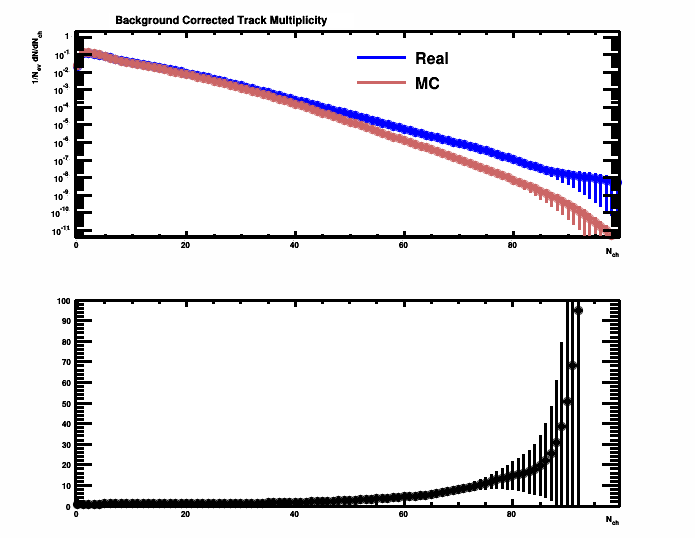
\includegraphics[width=\textwidth]{/afs/cern.ch/user/d/dvoong/cmtuser/DaVinci_v33r6/Phys/ChargedParticleMultiplicity/python/multiplicity/tracks/data_files/TrackMultiplicityPlottingJob/bk/Down/mc/-1/-1/bk/Down/mc/-1/-1/meissner_multiplicity_full/bk/Down/real/-1/-1/bk/Down/real/-1/-1/pngs/comparison/background_corrected/2-0_4-5_comparison.png}
%		\caption{$2.0 \le \eta \le 4.5$}
%	\end{subfigure}
%	\begin{subfigure}{0.32\textwidth}
%		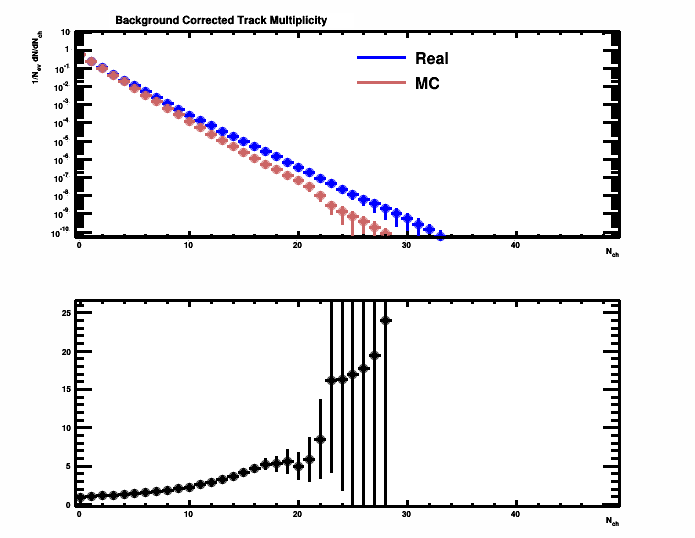
\includegraphics[width=\textwidth]{/afs/cern.ch/user/d/dvoong/cmtuser/DaVinci_v33r6/Phys/ChargedParticleMultiplicity/python/multiplicity/tracks/data_files/TrackMultiplicityPlottingJob/bk/Down/mc/-1/-1/bk/Down/mc/-1/-1/meissner_multiplicity/bk/Down/real/-1/-1/bk/Down/real/-1/-1/pngs/comparison/background_corrected/2-0_2-5_comparison.png}
%		\caption{$2.0 \le \eta \le 2.5$}
%	\end{subfigure}
%	\begin{subfigure}{0.32\textwidth}
%		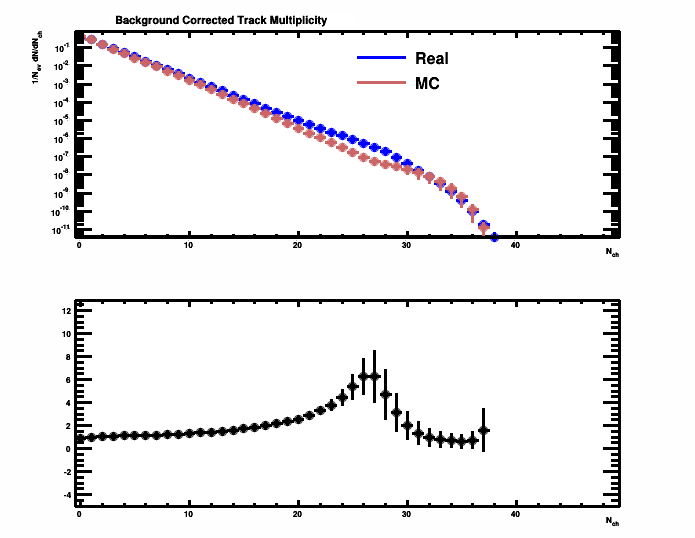
\includegraphics[width=\textwidth]{/afs/cern.ch/user/d/dvoong/cmtuser/DaVinci_v33r6/Phys/ChargedParticleMultiplicity/python/multiplicity/tracks/data_files/TrackMultiplicityPlottingJob/bk/Down/mc/-1/-1/bk/Down/mc/-1/-1/meissner_multiplicity/bk/Down/real/-1/-1/bk/Down/real/-1/-1/pngs/comparison/background_corrected/2-5_3-0_comparison.png}
%		\caption{$2.5 \le \eta \le 3.0$}
%	\end{subfigure}
%	\begin{subfigure}{0.32\textwidth}
%		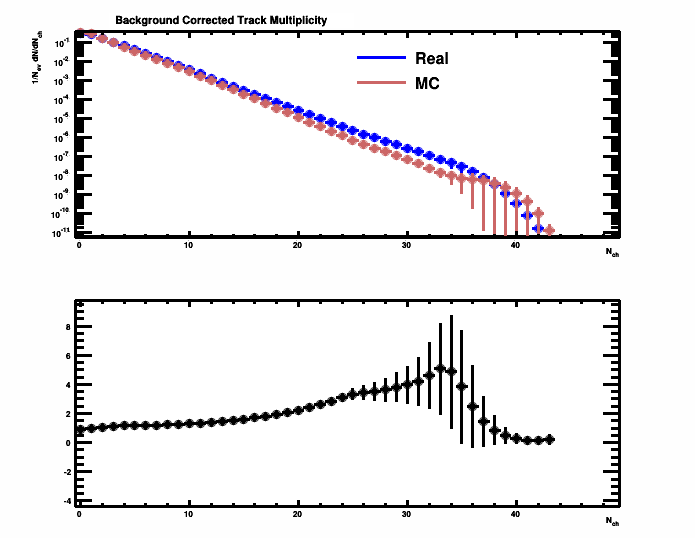
\includegraphics[width=\textwidth]{/afs/cern.ch/user/d/dvoong/cmtuser/DaVinci_v33r6/Phys/ChargedParticleMultiplicity/python/multiplicity/tracks/data_files/TrackMultiplicityPlottingJob/bk/Down/mc/-1/-1/bk/Down/mc/-1/-1/meissner_multiplicity/bk/Down/real/-1/-1/bk/Down/real/-1/-1/pngs/comparison/background_corrected/3-0_3-5_comparison.png}
%		\caption{$3.0 \le \eta \le 3.5$}
%	\end{subfigure}
%	\begin{subfigure}{0.32\textwidth}
%		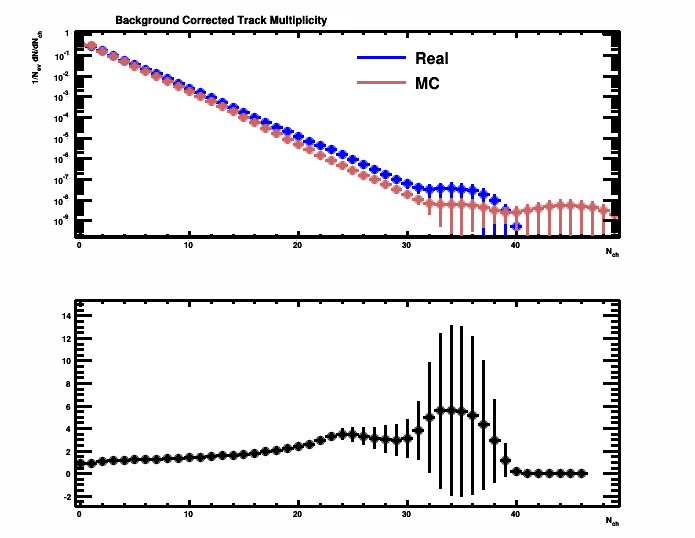
\includegraphics[width=\textwidth]{/afs/cern.ch/user/d/dvoong/cmtuser/DaVinci_v33r6/Phys/ChargedParticleMultiplicity/python/multiplicity/tracks/data_files/TrackMultiplicityPlottingJob/bk/Down/mc/-1/-1/bk/Down/mc/-1/-1/meissner_multiplicity/bk/Down/real/-1/-1/bk/Down/real/-1/-1/pngs/comparison/background_corrected/3-5_4-0_comparison.png}
%		\caption{$3.5 \le \eta \le 4.0$}
%	\end{subfigure}
%	\begin{subfigure}{0.32\textwidth}
%		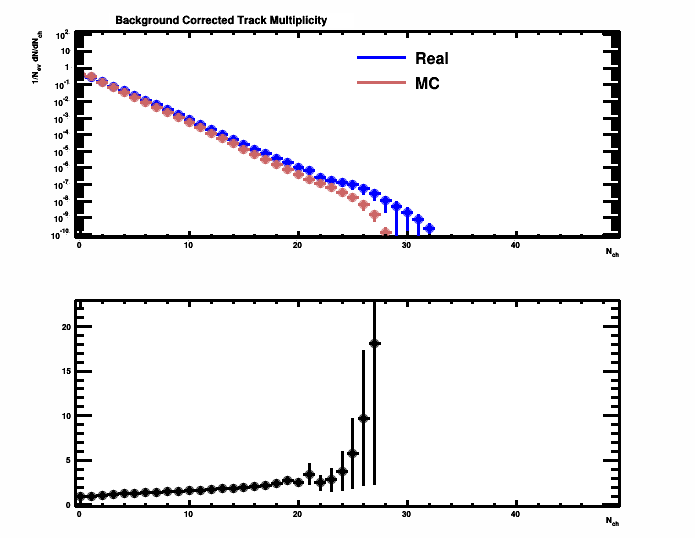
\includegraphics[width=\textwidth]{/afs/cern.ch/user/d/dvoong/cmtuser/DaVinci_v33r6/Phys/ChargedParticleMultiplicity/python/multiplicity/tracks/data_files/TrackMultiplicityPlottingJob/bk/Down/mc/-1/-1/bk/Down/mc/-1/-1/meissner_multiplicity/bk/Down/real/-1/-1/bk/Down/real/-1/-1/pngs/comparison/background_corrected/4-0_4-5_comparison.png}
%		\caption{$4.0 \le \eta \le 4.5$}
%	\end{subfigure}
%	\caption{Background corrected track multiplicities from real data and MC}
%	\label{fig: background corrected track multiplicity comparison}
%\end{figure}

\begin{figure}[H]
	\centering
	\begin{subfigure}{0.32\textwidth}
		\includegraphics[width=\textwidth]{Chapters/multiplicity/images/background_corrected/real/2-0_4-5_norm.png}
		\caption{$2.0 \le \eta \le 4.5$}
	\end{subfigure}
	\begin{subfigure}{0.32\textwidth}
		\includegraphics[width=\textwidth]{Chapters/multiplicity/images/background_corrected/real/2-0_2-5_norm.png}
		\caption{$2.0 \le \eta \le 2.5$}
	\end{subfigure}
	\begin{subfigure}{0.32\textwidth}
		\includegraphics[width=\textwidth]{Chapters/multiplicity/images/background_corrected/real/2-5_3-0_norm.png}
		\caption{$2.5 \le \eta \le 3.0$}
	\end{subfigure}
	\begin{subfigure}{0.32\textwidth}
		\includegraphics[width=\textwidth]{Chapters/multiplicity/images/background_corrected/real/3-0_3-5_norm.png}
		\caption{$3.0 \le \eta \le 3.5$}
	\end{subfigure}
	\begin{subfigure}{0.32\textwidth}
		\includegraphics[width=\textwidth]{Chapters/multiplicity/images/background_corrected/real/3-5_4-0_norm.png}
		\caption{$3.5 \le \eta \le 4.0$}
	\end{subfigure}
	\begin{subfigure}{0.32\textwidth}
		\includegraphics[width=\textwidth]{Chapters/multiplicity/images/background_corrected/real/4-0_4-5_norm.png}
		\caption{$4.0 \le \eta \le 4.5$}
	\end{subfigure}
	\caption{Background corrected track multiplicities in measured data}
	\label{fig: background corrected track multiplicities}
\end{figure}

\begin{figure}[H]
	\centering
	\begin{subfigure}{0.32\textwidth}
		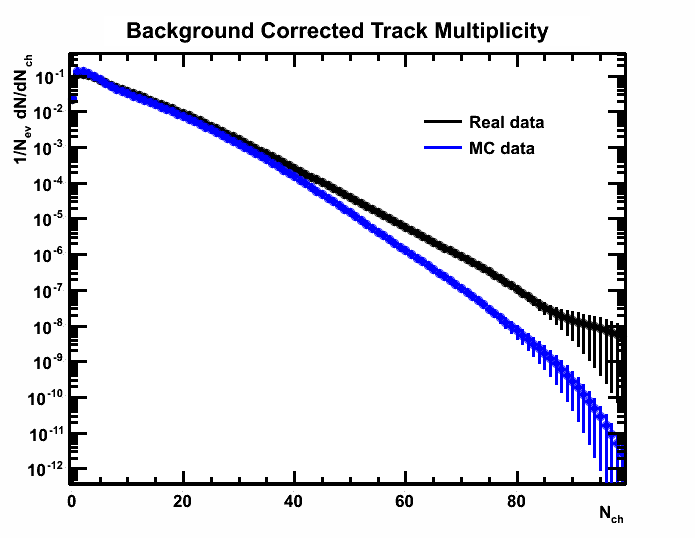
\includegraphics[width=\textwidth]{Chapters/multiplicity/charged_particle_event_multiplicity/images/background_correction_comparison/2_0-4_5.png}
		\caption{$2.0 \le \eta \le 4.5$}
	\end{subfigure}
	\begin{subfigure}{0.32\textwidth}
		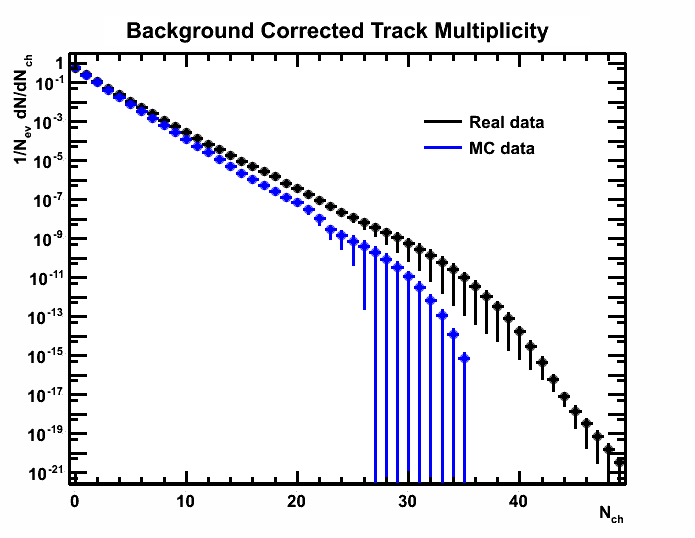
\includegraphics[width=\textwidth]{Chapters/multiplicity/charged_particle_event_multiplicity/images/background_correction_comparison/2_0-2_5.png}
		\caption{$2.0 \le \eta \le 2.5$}
	\end{subfigure}
	\begin{subfigure}{0.32\textwidth}
		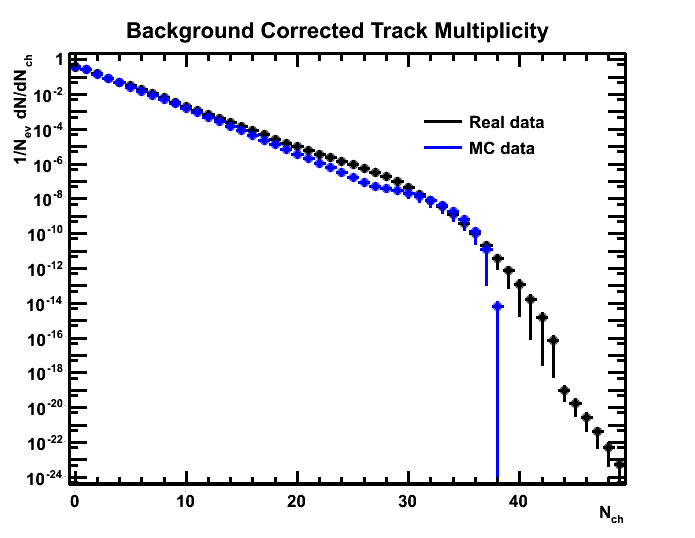
\includegraphics[width=\textwidth]{Chapters/multiplicity/charged_particle_event_multiplicity/images/background_correction_comparison/2_5-3_0.png}
		\caption{$2.5 \le \eta \le 3.0$}
	\end{subfigure}
	\begin{subfigure}{0.32\textwidth}
		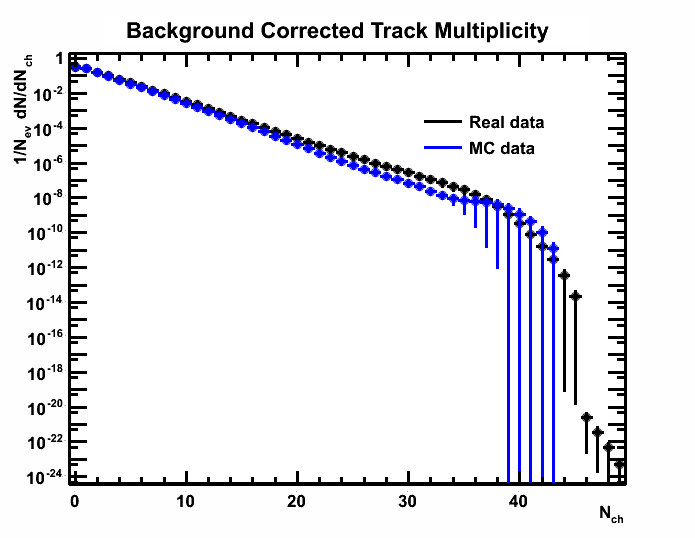
\includegraphics[width=\textwidth]{Chapters/multiplicity/charged_particle_event_multiplicity/images/background_correction_comparison/3_0-3_5.png}
		\caption{$3.0 \le \eta \le 3.5$}
	\end{subfigure}
	\begin{subfigure}{0.32\textwidth}
		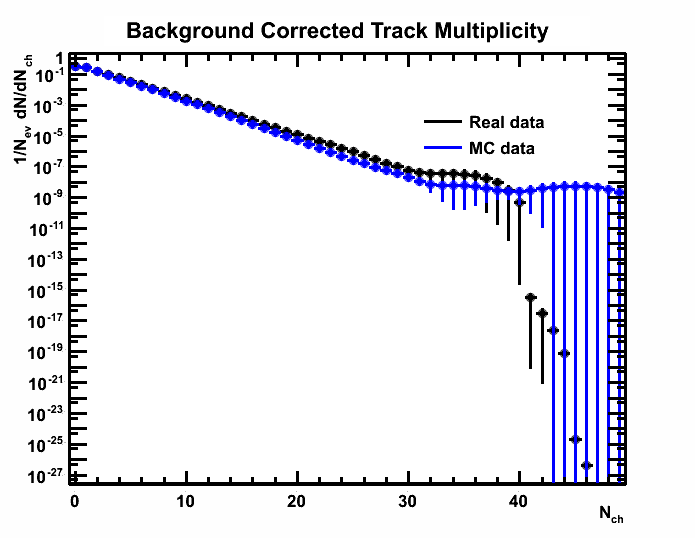
\includegraphics[width=\textwidth]{Chapters/multiplicity/charged_particle_event_multiplicity/images/background_correction_comparison/3_5-4_0.png}
		\caption{$3.5 \le \eta \le 4.0$}
	\end{subfigure}
	\begin{subfigure}{0.32\textwidth}
		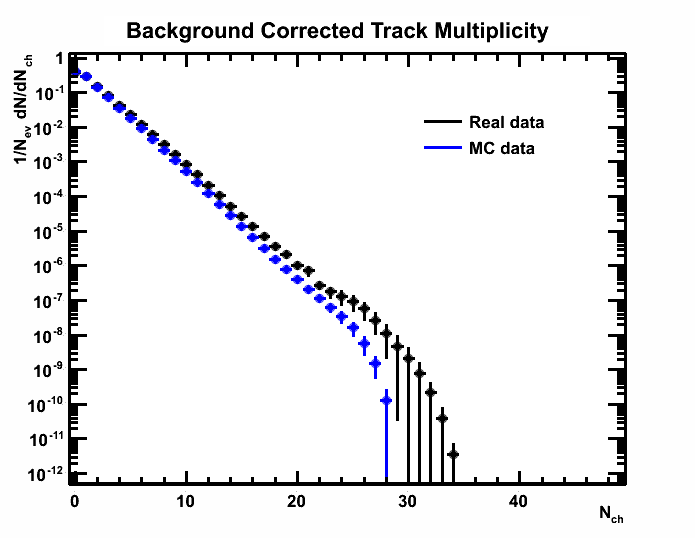
\includegraphics[width=\textwidth]{Chapters/multiplicity/charged_particle_event_multiplicity/images/background_correction_comparison/4_0-4_5.png}
		\caption{$4.0 \le \eta \le 4.5$}
	\end{subfigure}
	\caption{Background corrected track multiplicities from measured data and MC}
	\label{fig: background corrected track multiplicity comparison}
\end{figure}

%\begin{figure}[h]
%	\centering
%	\begin{subfigure}{0.32\textwidth}
%		\includegraphics[width=\textwidth]{/afs/cern.ch/user/d/dvoong/cmtuser/DaVinci_v33r6/Phys/ChargedParticleMultiplicity/python/multiplicity/tracks/data_files/TrackMultiplicityPlottingJob/bk/Down/mc/-1/-1/bk/Down/mc/-1/-1/meissner_multiplicity_full/bk/Down/mc/-1/-1/bk/Down/mc/-1/-1/pngs/cross_check/2-0_4-5.png}
%		\caption{$2.0 \le \eta \le 4.5$}
%	\end{subfigure}
%	\begin{subfigure}{0.32\textwidth}
%		\includegraphics[width=\textwidth]{/afs/cern.ch/user/d/dvoong/cmtuser/DaVinci_v33r6/Phys/ChargedParticleMultiplicity/python/multiplicity/tracks/data_files/TrackMultiplicityPlottingJob/bk/Down/mc/-1/-1/bk/Down/mc/-1/-1/meissner_multiplicity/bk/Down/mc/-1/-1/bk/Down/mc/-1/-1/pngs/cross_check/2-0_2-5.png}
%		\caption{$2.0 \le \eta \le 2.5$}
%	\end{subfigure}
%	\begin{subfigure}{0.32\textwidth}
%		\includegraphics[width=\textwidth]{/afs/cern.ch/user/d/dvoong/cmtuser/DaVinci_v33r6/Phys/ChargedParticleMultiplicity/python/multiplicity/tracks/data_files/TrackMultiplicityPlottingJob/bk/Down/mc/-1/-1/bk/Down/mc/-1/-1/meissner_multiplicity/bk/Down/mc/-1/-1/bk/Down/mc/-1/-1/pngs/cross_check/2-5_3-0.png}
%		\caption{$2.5 \le \eta \le 3.0$}
%	\end{subfigure}
%	\begin{subfigure}{0.32\textwidth}
%		\includegraphics[width=\textwidth]{/afs/cern.ch/user/d/dvoong/cmtuser/DaVinci_v33r6/Phys/ChargedParticleMultiplicity/python/multiplicity/tracks/data_files/TrackMultiplicityPlottingJob/bk/Down/mc/-1/-1/bk/Down/mc/-1/-1/meissner_multiplicity/bk/Down/mc/-1/-1/bk/Down/mc/-1/-1/pngs/cross_check/3-0_3-5.png}
%		\caption{$3.0 \le \eta \le 3.5$}
%	\end{subfigure}
%	\begin{subfigure}{0.32\textwidth}
%		\includegraphics[width=\textwidth]{/afs/cern.ch/user/d/dvoong/cmtuser/DaVinci_v33r6/Phys/ChargedParticleMultiplicity/python/multiplicity/tracks/data_files/TrackMultiplicityPlottingJob/bk/Down/mc/-1/-1/bk/Down/mc/-1/-1/meissner_multiplicity/bk/Down/mc/-1/-1/bk/Down/mc/-1/-1/pngs/cross_check/3-5_4-0.png}
%		\caption{$3.5 \le \eta \le 4.0$}
%	\end{subfigure}
%	\begin{subfigure}{0.32\textwidth}
%		\includegraphics[width=\textwidth]{/afs/cern.ch/user/d/dvoong/cmtuser/DaVinci_v33r6/Phys/ChargedParticleMultiplicity/python/multiplicity/tracks/data_files/TrackMultiplicityPlottingJob/bk/Down/mc/-1/-1/bk/Down/mc/-1/-1/meissner_multiplicity/bk/Down/mc/-1/-1/bk/Down/mc/-1/-1/pngs/cross_check/4-0_4-5.png}
%		\caption{$4.0 \le \eta \le 4.5$}
%	\end{subfigure}
%	\caption{Background correction cross-check. Background corrected track multiplicities are compared with tracks matched to generator prompt particles by MC truth matching}
%	\label{fig: background corrected track multiplicity cross-check}
%\end{figure}
\subsection{Efficiency Correction}
\label{subsection: charged particle multiplicity, efficiency correction}

\section{Response Matrix}
\label{section: response matrix}

The response matrix is an n by m matrix $R_{nm}$, each element gives the probability of reconstructing n number of tracks given an event with m number of particles. The relationship between the reconstructed track multiplicity  and true particle distribution ($a$) is described by the equation,

\begin{equation}
	a = R \cdot b
\end{equation} 

where a and b are column matrices describing the track and particle multiplicities respectively such that $a_i$ is the number of events with $i$ reconstructed tracks and $b_j$ is the number of events with $j$ corresponding true particles.

The response matrix is determined using truth information from Monte Carlo simulated events. 

\begin{figure}
	\centering
	\begin{subfigure}{0.32\textwidth}
		\includegraphics[width=\textwidth]{/afs/cern.ch/user/d/dvoong/cmtuser/DaVinci_v33r6/Phys/ChargedParticleMultiplicity/python/response_matrix/data_files/ResponseMatrixPlottingJob/bk/Down/mc/-1/-1/bk/Down/mc/-1/-1/meissner_multiplicity_full/bk/Down/mc/-1/-1/bk/Down/mc/-1/-1/pngs/background_corrected/2-0_4-5.png}
		\caption{$2.0 \le \eta \le 4.5$}
	\end{subfigure}
	\begin{subfigure}{0.32\textwidth}
		\includegraphics[width=\textwidth]{/afs/cern.ch/user/d/dvoong/cmtuser/DaVinci_v33r6/Phys/ChargedParticleMultiplicity/python/response_matrix/data_files/ResponseMatrixPlottingJob/bk/Down/mc/-1/-1/bk/Down/mc/-1/-1/meissner_multiplicity/bk/Down/mc/-1/-1/bk/Down/mc/-1/-1/pngs/background_corrected/2-0_2-5.png}
		\caption{$2.0 \le \eta \le 2.5$}
	\end{subfigure}
	\begin{subfigure}{0.32\textwidth}
		\includegraphics[width=\textwidth]{/afs/cern.ch/user/d/dvoong/cmtuser/DaVinci_v33r6/Phys/ChargedParticleMultiplicity/python/response_matrix/data_files/ResponseMatrixPlottingJob/bk/Down/mc/-1/-1/bk/Down/mc/-1/-1/meissner_multiplicity/bk/Down/mc/-1/-1/bk/Down/mc/-1/-1/pngs/background_corrected/2-5_3-0.png}
		\caption{$2.5 \le \eta \le 3.0$}
	\end{subfigure}
	\begin{subfigure}{0.32\textwidth}
		\includegraphics[width=\textwidth]{/afs/cern.ch/user/d/dvoong/cmtuser/DaVinci_v33r6/Phys/ChargedParticleMultiplicity/python/response_matrix/data_files/ResponseMatrixPlottingJob/bk/Down/mc/-1/-1/bk/Down/mc/-1/-1/meissner_multiplicity/bk/Down/mc/-1/-1/bk/Down/mc/-1/-1/pngs/background_corrected/3-0_3-5.png}
		\caption{$3.0 \le \eta \le 3.5$}
	\end{subfigure}
	\begin{subfigure}{0.32\textwidth}
		\includegraphics[width=\textwidth]{/afs/cern.ch/user/d/dvoong/cmtuser/DaVinci_v33r6/Phys/ChargedParticleMultiplicity/python/response_matrix/data_files/ResponseMatrixPlottingJob/bk/Down/mc/-1/-1/bk/Down/mc/-1/-1/meissner_multiplicity/bk/Down/mc/-1/-1/bk/Down/mc/-1/-1/pngs/background_corrected/3-5_4-0.png}
		\caption{$3.5 \le \eta \le 4.0$}
	\end{subfigure}
	\begin{subfigure}{0.32\textwidth}
		\includegraphics[width=\textwidth]{/afs/cern.ch/user/d/dvoong/cmtuser/DaVinci_v33r6/Phys/ChargedParticleMultiplicity/python/response_matrix/data_files/ResponseMatrixPlottingJob/bk/Down/mc/-1/-1/bk/Down/mc/-1/-1/meissner_multiplicity/bk/Down/mc/-1/-1/bk/Down/mc/-1/-1/pngs/background_corrected/4-0_4-5.png}
		\caption{$4.0 \le \eta \le 4.5$}
	\end{subfigure}
	\caption{Background corrected response matrices}
	\label{fig: background corrected response matrices}
\end{figure}
\subsubsection{True Multiplicity Parameterisation}
\label{subsection: charged particle event multiplicity, true multiplicity parameterisation}

Starting from equation \ref{equation: multiplicity-response relationship} a heuristic approach to calculating the true particle multiplicity can be employed. By making a educated guess at the shape of the true distribution a corresponding expected multiplicity can be calculated by applying the response matrix. Comparing the observed multiplicity to the expected multiplicity gives a quantifiable measurement of the accuracy of the guess. To achieve this in a more systematic way, a parameterisation of the true distribution ($b'$) can be made for which a corresponding response (or smearing) functions ($a'$) exists. By fitting the response function to the observed multiplicity the associated parameters can be propagated back in terms of the parameterisation of the true multiplicity distribution to give a corrected multiplicity distribution. The response function and corresponding $\chi^2$ minimisation function that were used are,

\begin{equation}
	a'(p_0, p_1, ..., p_n) = R \cdot b'(p_0, p_1, ..., p_n)
\end{equation}

\begin{equation}
	\chi^2(p_0, p_1, ..., p_n) = \sum^{N_\mathrm{max}}_{N_\mathrm{ch}} \sqrt{a(N_\mathrm{ch})^2 - a'(N_\mathrm{ch})^2}
	\label{equation: response function minimisation}
\end{equation}

Where $p_0, p_1, ..., p_n$ corresponds to the parameters used to parameterise the response function and hence true multiplicity, $N_\mathrm{max}$ is the maximum number of reconstructed tracks ($N_\mathrm{ch}$), $a(N_\mathrm{ch})$ is the number of events with $N_\mathrm{ch}$ tracks and $a'(N_\mathrm{ch})$ is the number of events with $N_\mathrm{ch}$ reconstructed tracks predicted by the response function.

%The true multiplicity is parameterised using several functions in order to optimise the robustness of the unfolding procedure.
%The following parameterisation functions were used,

The true multiplicity distribution is parameterised by several parameterisations (listed below). These parameterisations consist of several parameters such that the parameterisations are extremely flexible and robust. This enables the parameterisations to model a range of possible true distributions, minimising the bias associated to modelling an unknown distribution. The initial values of the parameters in each parameterisation are initialised by fitting MC generated data with each parameterisations, the fits are shown in figure \ref{fig: parameterisation fits} and the parameters are shown in table \ref{table: gen multiplicity parameters}.

\begin{itemize}
	\item $P_A(x) = p_0 e^{p_1x}x^2 + e^{p_2x}x^2$
	\item $P_B(x) = e^{p_0 + p_1x} \cdot (x + 1)^3 + e^{p_2 + p_3x} \cdot x^2 + e^{p_4 + p_5x} \cdot x^2$
%	\item $P_C(x) = \mathrm{NBD}(x; p_0, p_1) + p_6 \mathrm{NBD}(x + p_8; p_2, p_3) + p_7 \mathrm{NBD}(x + p_9; p_4, p_5)$
	\item $P_C(x) = e^{p_0 + p_1x} \cdot x^{p_2} + e^{p_3 + p_4x} \cdot x^{p_5} + e^{p_6 + p_7x} \cdot x^{p_8}$
%	\item $P_D(x) = e^{p_0 + p_1 \cdot x^{p_2}} \cdot x^2 + e^{p_3 + p_4x + p_5(p_7x)^{p_6}} + \frac{p_8}{x+1} \cdot e^\frac{p9}{x+1}$
	\item $P_E(x) = e^{p_0 + p_1x} \cdot x^{p_2} + e^{p_3 + p_4x} \cdot x^2$
\end{itemize}

%\begin{equation}
%	f(x) = p_0 e^{p_1x}x^2 + e^{p_2x}x^2
%\end{equation}
%
%\begin{equation}
%	f(x) = e^{p_0 + p_1x} \cdot (x + 1)^3 + e^{p_2 + p_3x} \cdot x^2 + e^{p_4 + p_5x} \cdot x^2
%\end{equation}
%
%\begin{equation}
%	f(x) = \frac{n!}{x!(n-x)!} \cdot p^x \cdot (1-p)^{n-x} + p_6 \cdot \left( \frac{n'!}{x!(n'-x)!} \cdot p'^x \cdot(1-p')^{n'-x} \right) + p_7 \cdot \left( \frac{n''!}{(x+1)!(n''-x)!} \cdot p''^{x + 1} \cdot (1-p'')^{(n'' - (x+1))} \right)
%\end{equation}
%
%\begin{equation}
%	f(x) = e^{p_0 + p_1x} \cdot x^{p_2} + e^{p_3 + p_4x} \cdot x^{p_5} + e^{p_6 + p_7x} \cdot x^{p_8}
%\end{equation}
%
%\begin{equation}
%	f(x) = e^{p_0 + p_1 \cdot x^{p_2}} \cdot x^2 + e^{p_3 + p_4x + p_5(p_7x)^{p_6}} + \frac{p_8}{x+1} \cdot e^\frac{p9}{x+1}
%\end{equation}
%
%\begin{equation}
%	f(x) = e^{p_0 + p_1x} \cdot x^{p_2} + e^{p_3 + p_4x} \cdot x^2
%\end{equation}

%Due to the non-perturbative nature of the multiplicity distribution there is ambiguity in the shape of the multiplicity distribution. These parameterisation functions are adopted in order to give a high degree of flexibility and robustness in describing the multiplicity distribution.

\begin{figure}[H]
	\centering
	\begin{subfigure}{0.49\textwidth}
		\includegraphics[width=\textwidth]{/afs/cern.ch/user/d/dvoong/cmtuser/DaVinci_v33r6/Phys/ChargedParticleMultiplicity/python/multiplicity/genps/parameterisation/data_files/GenpMultiplicityParameterisationPlottingJob/bk/Down/mc/-1/-1/bk/Down/mc/-1/155/parameterisation_a/2_0-4_5/parameterisation_a.png}
		\caption{Parameterisation A}
		\label{}
	\end{subfigure}
	\begin{subfigure}{0.49\textwidth}
		\includegraphics[width=\textwidth]{/afs/cern.ch/user/d/dvoong/cmtuser/DaVinci_v33r6/Phys/ChargedParticleMultiplicity/python/multiplicity/genps/parameterisation/data_files/GenpMultiplicityParameterisationPlottingJob/bk/Down/mc/-1/-1/bk/Down/mc/-1/155/parameterisation_b/2_0-4_5/parameterisation_b.png}
		\caption{Parameterisation B}
		\label{}
	\end{subfigure}
%	\begin{subfigure}{0.49\textwidth}
%		\includegraphics[width=\textwidth]{/afs/cern.ch/user/d/dvoong/cmtuser/DaVinci_v33r6/Phys/ChargedParticleMultiplicity/python/multiplicity/genps/parameterisation/data_files/GenpMultiplicityParameterisationPlottingJob/bk/Down/mc/-1/-1/bk/Down/mc/-1/155/parameterisation_c/2_0-4_5/parameterisation_c.png}
%		\caption{Parameterisation C}
%		\label{}
%	\end{subfigure}
	\begin{subfigure}{0.49\textwidth}
		\includegraphics[width=\textwidth]{/afs/cern.ch/user/d/dvoong/cmtuser/DaVinci_v33r6/Phys/ChargedParticleMultiplicity/python/multiplicity/genps/parameterisation/data_files/GenpMultiplicityParameterisationPlottingJob/bk/Down/mc/-1/-1/bk/Down/mc/-1/155/parameterisation_d/2_0-4_5/parameterisation_d.png}
		\caption{Parameterisation D}
		\label{}
	\end{subfigure}
%	\begin{subfigure}{0.49\textwidth}
%		\includegraphics[width=\textwidth]{/afs/cern.ch/user/d/dvoong/cmtuser/DaVinci_v33r6/Phys/ChargedParticleMultiplicity/python/multiplicity/genps/parameterisation/data_files/GenpMultiplicityParameterisationPlottingJob/bk/Down/mc/-1/-1/bk/Down/mc/-1/155/parameterisation_e/2_0-4_5/parameterisation_e.png}
%		\caption{Parameterisation E}
%		\label{}
%	\end{subfigure}
	\begin{subfigure}{0.49\textwidth}
		\includegraphics[width=\textwidth]{/afs/cern.ch/user/d/dvoong/cmtuser/DaVinci_v33r6/Phys/ChargedParticleMultiplicity/python/multiplicity/genps/parameterisation/data_files/GenpMultiplicityParameterisationPlottingJob/bk/Down/mc/-1/-1/bk/Down/mc/-1/155/parameterisation_f/2_0-4_5/parameterisation_f.png}
		\caption{Parameterisation F}
		\label{}
	\end{subfigure}
	\caption{Parameterisation fits to MC data for $2.0 \le \eta \le 4.5$. The solid blue line corresponds to the total fit and the dotted lines correspond to the components of the total fit}
	\label{fig: parameterisation fits}
\end{figure}

\newpage
\begin{table}[h]
	\caption{True multiplicity parameterisations fit to generated prompt particle distributions}
	\label{table: gen multiplicity parameters}
	\begin{subtable}{0.49\textwidth}
		\caption{Parameterisation A}
		\centering
		\begin{tabular}{|c|c|}
			\centering
			p0 & $14.414 \pm 0.988$ \\
			p1 & $-0.19995 \pm 0.181$ \\
			p2 & $17.887 \pm 0.989$ \\
			p3 & $-0.60499 \pm 0.832$ \\
			p4 & $0.01735 \pm 0.332$ \\
			p5 & $1.5373 \pm 0.998$ \\
			p6 & $1.3577 \pm 1.0$ \\
		\end{tabular}
	\end{subtable}
	\begin{subtable}{0.49\textwidth}
		\caption{Parameterisation B}
		\centering
		\begin{tabular}{|c|c|}
			\centering
			p0 & $-4.4678 \pm 33.9$ \\
			p1 & $-0.66946 \pm 2.78$ \\
			p2 & $-2.7404 \pm 53.7$ \\
			p3 & $-1.0328 \pm 11.9$ \\
			p4 & $-6.0631 \pm 33.0$ \\
			p5 & $-0.19869 \pm 0.323$ \\
		\end{tabular}
	\end{subtable}
%	\begin{subtable}{0.49\textwidth}
%		\caption{Parameterisation C}
%		\centering
%		\begin{tabular}{|c|c|}
%			\centering
%			p0 & $1.1237 \pm 3.91$ \\
%			p1 & $0.090301 \pm 0.76$ \\
%			p2 & $23.184 \pm 6.7e+02$ \\
%			p3 & $0.84887 \pm 0.618$ \\
%			p4 & $4.2472 \pm 43.1$ \\
%			p5 & $0.12728 \pm 0.628$ \\
%			p6 & $0.20308 \pm 0.662$ \\
%			p7 & $-0.10058 \pm 1.45$ \\
%		\end{tabular}
%	\end{subtable}
	\begin{subtable}{0.49\textwidth}
		\caption{Parameterisation D}
		\centering
		\begin{tabular}{|c|c|}
			\centering
			p0 & $-17.893 \pm 1.0$ \\
			p1 & $-0.33501 \pm 0.198$ \\
			p2 & $4.1461 \pm 1.04$ \\
			p3 & $-9.5155 \pm 0.993$ \\
			p4 & $-0.22568 \pm 0.178$ \\
			p5 & $3.1305 \pm 0.962$ \\
			p6 & $-2.5895 \pm 0.994$ \\
			p7 & $-0.37285 \pm 0.531$ \\
			p8 & $1.1071 \pm 0.97$ \\
		\end{tabular}
	\end{subtable}
%	\begin{subtable}{0.49\textwidth}
%		\caption{Parameterisation E}
%		\centering
%		\begin{tabular}{|c|c|}
%			\centering
%			p0 & $-6.9649 \pm 11.9$ \\
%			p1 & $-0.1352 \pm 0.302$ \\
%			p2 & $1.074 \pm 0.559$ \\
%			p3 & $16.049 \pm 11.8$ \\
%			p4 & $-0.39655 \pm 0.912$ \\
%			p5 & $-9.7608 \pm 6.69$ \\
%			p6 & $-0.066749 \pm 0.0762$ \\
%			p7 & $7.3009e-05 \pm 0.000732$ \\
%			p8 & $-101.39 \pm 6.09e+04$ \\
%			p9 & $-837.68 \pm 4.06e+04$ \\
%		\end{tabular}
%	\end{subtable}
	\begin{subtable}{0.49\textwidth}
		\caption{Parameterisation F}
		\centering
		\begin{tabular}{|c|c|}
			\centering
			p0 & $-6.3713 \pm 33.5$ \\
			p1 & $-0.20009 \pm 0.272$ \\
			p2 & $-2.6787 \pm 33.5$ \\
			p3 & $-0.6491 \pm 1.08$ \\
		\end{tabular}
	\end{subtable}
\end{table}
\newpage

%The response functions for the background corrected multiplicities in figure \ref{fig: background corrected track multiplicities} and parameterisations in figure \ref{fig: parameterisation fits} are shown in figure \ref{fig: response function, measured data} and \ref{fig: response function, mc data} for measured and MC data. The corresponding unfolded multiplicities are shown figure \ref{fig: unfolded multiplicity, measured data} and \ref{fig: unfolded multiplicity, mc data} respectively.

The response functions for the background corrected multiplicities in figure \ref{fig: background corrected track multiplicities} and parameterisations in figure \ref{fig: parameterisation fits} are shown in figure \ref{fig: response function, measured data} for measured data. The corresponding unfolded multiplicities are shown figure \ref{fig: unfolded multiplicity, measured data}.

\begin{figure}[H]
	\centering
	\begin{subfigure}{0.49\textwidth}
		\includegraphics[width=\textwidth]{/afs/cern.ch/user/d/dvoong/cmtuser/DaVinci_v33r6/Phys/ChargedParticleMultiplicity/python/multiplicity/tracks/unfolding/data_files/UnfoldingPlottingWithStatsJob/bk/Down/mc/-1/-1/bk/Down/mc/-1/-1/meissner_multiplicity_full/bk/Down/real/-1/-1/bk/Down/real/-1/-1/bk/Down/mc/-1/-1/bk/Down/mc/-1/155/parameterisation_a/2_0-4_5/bk/Down/mc/-1/-1/bk/Down/mc/-1/-1/meissner_multiplicity_full/bk/Down/mc/-1/-1/bk/Down/mc/-1/-1/background_corrected/truncation/response_function.png}
		\caption{Parameterisation A}
	\end{subfigure}
	\begin{subfigure}{0.49\textwidth}
		\includegraphics[width=\textwidth]{/afs/cern.ch/user/d/dvoong/cmtuser/DaVinci_v33r6/Phys/ChargedParticleMultiplicity/python/multiplicity/tracks/unfolding/data_files/UnfoldingPlottingWithStatsJob/bk/Down/mc/-1/-1/bk/Down/mc/-1/-1/meissner_multiplicity_full/bk/Down/real/-1/-1/bk/Down/real/-1/-1/bk/Down/mc/-1/-1/bk/Down/mc/-1/155/parameterisation_b/2_0-4_5/bk/Down/mc/-1/-1/bk/Down/mc/-1/-1/meissner_multiplicity_full/bk/Down/mc/-1/-1/bk/Down/mc/-1/-1/background_corrected/truncation/response_function.png}
		\caption{Parameterisation B}
	\end{subfigure}
%	\begin{subfigure}{0.49\textwidth}
%		\includegraphics[width=\textwidth]{/afs/cern.ch/user/d/dvoong/cmtuser/DaVinci_v33r6/Phys/ChargedParticleMultiplicity/python/multiplicity/tracks/unfolding/data_files/UnfoldingPlottingWithStatsJob/bk/Down/mc/-1/-1/bk/Down/mc/-1/-1/meissner_multiplicity_full/bk/Down/real/-1/-1/bk/Down/real/-1/-1/bk/Down/mc/-1/-1/bk/Down/mc/-1/155/parameterisation_c/2_0-4_5/bk/Down/mc/-1/-1/bk/Down/mc/-1/-1/meissner_multiplicity_full/bk/Down/mc/-1/-1/bk/Down/mc/-1/-1/background_corrected/truncation/response_function.png}
%		\caption{Parameterisation C}
%	\end{subfigure}
	\begin{subfigure}{0.49\textwidth}
		\includegraphics[width=\textwidth]{/afs/cern.ch/user/d/dvoong/cmtuser/DaVinci_v33r6/Phys/ChargedParticleMultiplicity/python/multiplicity/tracks/unfolding/data_files/UnfoldingPlottingWithStatsJob/bk/Down/mc/-1/-1/bk/Down/mc/-1/-1/meissner_multiplicity_full/bk/Down/real/-1/-1/bk/Down/real/-1/-1/bk/Down/mc/-1/-1/bk/Down/mc/-1/155/parameterisation_d/2_0-4_5/bk/Down/mc/-1/-1/bk/Down/mc/-1/-1/meissner_multiplicity_full/bk/Down/mc/-1/-1/bk/Down/mc/-1/-1/background_corrected/truncation/response_function.png}
		\caption{Parameterisation D}
	\end{subfigure}
%	\begin{subfigure}{0.49\textwidth}
%		\includegraphics[width=\textwidth]{/afs/cern.ch/user/d/dvoong/cmtuser/DaVinci_v33r6/Phys/ChargedParticleMultiplicity/python/multiplicity/tracks/unfolding/data_files/UnfoldingPlottingWithStatsJob/bk/Down/mc/-1/-1/bk/Down/mc/-1/-1/meissner_multiplicity_full/bk/Down/real/-1/-1/bk/Down/real/-1/-1/bk/Down/mc/-1/-1/bk/Down/mc/-1/155/parameterisation_e/2_0-4_5/bk/Down/mc/-1/-1/bk/Down/mc/-1/-1/meissner_multiplicity_full/bk/Down/mc/-1/-1/bk/Down/mc/-1/-1/background_corrected/truncation/response_function.png}
%		\caption{Parameterisation E}
%	\end{subfigure}
	\begin{subfigure}{0.49\textwidth}
		\includegraphics[width=\textwidth]{/afs/cern.ch/user/d/dvoong/cmtuser/DaVinci_v33r6/Phys/ChargedParticleMultiplicity/python/multiplicity/tracks/unfolding/data_files/UnfoldingPlottingWithStatsJob/bk/Down/mc/-1/-1/bk/Down/mc/-1/-1/meissner_multiplicity_full/bk/Down/real/-1/-1/bk/Down/real/-1/-1/bk/Down/mc/-1/-1/bk/Down/mc/-1/155/parameterisation_f/2_0-4_5/bk/Down/mc/-1/-1/bk/Down/mc/-1/-1/meissner_multiplicity_full/bk/Down/mc/-1/-1/bk/Down/mc/-1/-1/background_corrected/truncation/response_function.png}
		\caption{Parameterisation F}
	\end{subfigure}
	\caption{Response Function for $2.0 \le \eta \le 4.5$, Measured Data}
	\label{fig: response function, measured data}
\end{figure}

%\newpage
\begin{table}
	\centering
	\caption{Response function parameters}
	\label{table: response function parameters}
	\begin{subtable}{0.49\textwidth}
		\centering
		\caption{Parameterisation A}
		\input{/afs/cern.ch/user/d/dvoong/cmtuser/DaVinci_v33r6/Phys/ChargedParticleMultiplicity/python/multiplicity/tracks/unfolding/data_files/UnfoldingPlottingWithStatsJob/bk/Down/mc/-1/-1/bk/Down/mc/-1/-1/meissner_multiplicity_full/bk/Down/mc/-1/-1/bk/Down/mc/-1/155/bk/Down/mc/-1/-1/bk/Down/mc/-1/155/parameterisation_a/2_0-4_5/bk/Down/mc/-1/-1/bk/Down/mc/-1/-1/meissner_multiplicity_full/bk/Down/mc/-1/-1/bk/Down/mc/-1/-1/background_corrected/parameterised/parameters}
	\end{subtable}
	\begin{subtable}{0.49\textwidth}
		\centering
		\caption{Parameterisation B}
		\input{/afs/cern.ch/user/d/dvoong/cmtuser/DaVinci_v33r6/Phys/ChargedParticleMultiplicity/python/multiplicity/tracks/unfolding/data_files/UnfoldingPlottingWithStatsJob/bk/Down/mc/-1/-1/bk/Down/mc/-1/-1/meissner_multiplicity_full/bk/Down/mc/-1/-1/bk/Down/mc/-1/155/bk/Down/mc/-1/-1/bk/Down/mc/-1/155/parameterisation_b/2_0-4_5/bk/Down/mc/-1/-1/bk/Down/mc/-1/-1/meissner_multiplicity_full/bk/Down/mc/-1/-1/bk/Down/mc/-1/-1/background_corrected/parameterised/parameters}
	\end{subtable}
	\begin{subtable}{0.49\textwidth}
		\caption{Parameterisation D}
		\centering
		\input{/afs/cern.ch/user/d/dvoong/cmtuser/DaVinci_v33r6/Phys/ChargedParticleMultiplicity/python/multiplicity/tracks/unfolding/data_files/UnfoldingPlottingWithStatsJob/bk/Down/mc/-1/-1/bk/Down/mc/-1/-1/meissner_multiplicity_full/bk/Down/mc/-1/-1/bk/Down/mc/-1/155/bk/Down/mc/-1/-1/bk/Down/mc/-1/155/parameterisation_d/2_0-4_5/bk/Down/mc/-1/-1/bk/Down/mc/-1/-1/meissner_multiplicity_full/bk/Down/mc/-1/-1/bk/Down/mc/-1/-1/background_corrected/parameterised/parameters}
	\end{subtable}
%	\begin{subtable}{0.49\textwidth}
%		\centering
%		\caption{Parameterisation E}
%		\input{/afs/cern.ch/user/d/dvoong/cmtuser/DaVinci_v33r6/Phys/ChargedParticleMultiplicity/python/multiplicity/tracks/unfolding/data_files/UnfoldingPlottingWithStatsJob/bk/Down/mc/-1/-1/bk/Down/mc/-1/-1/meissner_multiplicity_full/bk/Down/mc/-1/-1/bk/Down/mc/-1/155/bk/Down/mc/-1/-1/bk/Down/mc/-1/155/parameterisation_e/2_0-4_5/bk/Down/mc/-1/-1/bk/Down/mc/-1/-1/meissner_multiplicity_full/bk/Down/mc/-1/-1/bk/Down/mc/-1/-1/background_corrected/parameterised/parameters}
%	\end{subtable}
	\begin{subtable}{0.49\textwidth}
		\centering
		\caption{Parameterisation F}
		\input{/afs/cern.ch/user/d/dvoong/cmtuser/DaVinci_v33r6/Phys/ChargedParticleMultiplicity/python/multiplicity/tracks/unfolding/data_files/UnfoldingPlottingWithStatsJob/bk/Down/mc/-1/-1/bk/Down/mc/-1/-1/meissner_multiplicity_full/bk/Down/mc/-1/-1/bk/Down/mc/-1/155/bk/Down/mc/-1/-1/bk/Down/mc/-1/155/parameterisation_f/2_0-4_5/bk/Down/mc/-1/-1/bk/Down/mc/-1/-1/meissner_multiplicity_full/bk/Down/mc/-1/-1/bk/Down/mc/-1/-1/background_corrected/parameterised/parameters}
	\end{subtable}
\end{table}
%\newpage

\begin{figure}[H]
	\centering
	\begin{subfigure}{0.49\textwidth}
		\includegraphics[width=\textwidth]{/afs/cern.ch/user/d/dvoong/cmtuser/DaVinci_v33r6/Phys/ChargedParticleMultiplicity/python/multiplicity/tracks/unfolding/data_files/UnfoldingPlottingWithStatsJob/bk/Down/mc/-1/-1/bk/Down/mc/-1/-1/meissner_multiplicity_full/bk/Down/real/-1/-1/bk/Down/real/-1/-1/bk/Down/mc/-1/-1/bk/Down/mc/-1/155/parameterisation_a/2_0-4_5/bk/Down/mc/-1/-1/bk/Down/mc/-1/-1/meissner_multiplicity_full/bk/Down/mc/-1/-1/bk/Down/mc/-1/-1/background_corrected/truncation/unfolded_multiplicity}
		\caption{Parameterisation A}
	\end{subfigure}
	\begin{subfigure}{0.49\textwidth}
		\includegraphics[width=\textwidth]{/afs/cern.ch/user/d/dvoong/cmtuser/DaVinci_v33r6/Phys/ChargedParticleMultiplicity/python/multiplicity/tracks/unfolding/data_files/UnfoldingPlottingWithStatsJob/bk/Down/mc/-1/-1/bk/Down/mc/-1/-1/meissner_multiplicity_full/bk/Down/real/-1/-1/bk/Down/real/-1/-1/bk/Down/mc/-1/-1/bk/Down/mc/-1/155/parameterisation_b/2_0-4_5/bk/Down/mc/-1/-1/bk/Down/mc/-1/-1/meissner_multiplicity_full/bk/Down/mc/-1/-1/bk/Down/mc/-1/-1/background_corrected/truncation/unfolded_multiplicity}
		\caption{Parameterisation B}
	\end{subfigure}
%	\begin{subfigure}{0.49\textwidth}
%		\includegraphics[width=\textwidth]{/afs/cern.ch/user/d/dvoong/cmtuser/DaVinci_v33r6/Phys/ChargedParticleMultiplicity/python/multiplicity/tracks/unfolding/data_files/UnfoldingPlottingJob/bk/Down/mc/-1/-1/bk/Down/mc/-1/-1/meissner_multiplicity_full/bk/Down/real/-1/-1/bk/Down/real/-1/-1/bk/Down/mc/-1/-1/bk/Down/mc/-1/-1/parameterisation_c/2_0-4_5/bk/Down/mc/-1/-1/bk/Down/mc/-1/-1/meissner_multiplicity_full/bk/Down/mc/-1/-1/bk/Down/mc/-1/-1/background_corrected/pngs/unfolded_multiplicity.png}
%		\caption{Parameterisation C}
%	\end{subfigure}
	\begin{subfigure}{0.49\textwidth}
		\includegraphics[width=\textwidth]{/afs/cern.ch/user/d/dvoong/cmtuser/DaVinci_v33r6/Phys/ChargedParticleMultiplicity/python/multiplicity/tracks/unfolding/data_files/UnfoldingPlottingWithStatsJob/bk/Down/mc/-1/-1/bk/Down/mc/-1/-1/meissner_multiplicity_full/bk/Down/real/-1/-1/bk/Down/real/-1/-1/bk/Down/mc/-1/-1/bk/Down/mc/-1/155/parameterisation_d/2_0-4_5/bk/Down/mc/-1/-1/bk/Down/mc/-1/-1/meissner_multiplicity_full/bk/Down/mc/-1/-1/bk/Down/mc/-1/-1/background_corrected/truncation/unfolded_multiplicity}
		\caption{Parameterisation D}
	\end{subfigure}
%	\begin{subfigure}{0.49\textwidth}
%		\includegraphics[width=\textwidth]{/afs/cern.ch/user/d/dvoong/cmtuser/DaVinci_v33r6/Phys/ChargedParticleMultiplicity/python/multiplicity/tracks/unfolding/data_files/UnfoldingPlottingWithStatsJob/bk/Down/mc/-1/-1/bk/Down/mc/-1/-1/meissner_multiplicity_full/bk/Down/real/-1/-1/bk/Down/real/-1/-1/bk/Down/mc/-1/-1/bk/Down/mc/-1/155/parameterisation_e/2_0-4_5/bk/Down/mc/-1/-1/bk/Down/mc/-1/-1/meissner_multiplicity_full/bk/Down/mc/-1/-1/bk/Down/mc/-1/-1/background_corrected/truncation/unfolded_multiplicity}
%		\caption{Parameterisation E}
%	\end{subfigure}
	\begin{subfigure}{0.49\textwidth}
		\includegraphics[width=\textwidth]{/afs/cern.ch/user/d/dvoong/cmtuser/DaVinci_v33r6/Phys/ChargedParticleMultiplicity/python/multiplicity/tracks/unfolding/data_files/UnfoldingPlottingWithStatsJob/bk/Down/mc/-1/-1/bk/Down/mc/-1/-1/meissner_multiplicity_full/bk/Down/real/-1/-1/bk/Down/real/-1/-1/bk/Down/mc/-1/-1/bk/Down/mc/-1/155/parameterisation_f/2_0-4_5/bk/Down/mc/-1/-1/bk/Down/mc/-1/-1/meissner_multiplicity_full/bk/Down/mc/-1/-1/bk/Down/mc/-1/-1/background_corrected/truncation/unfolded_multiplicity}
		\caption{Parameterisation F}
	\end{subfigure}
	\caption{Unfolded Multiplicity for $2.0 \le \eta \le 4.5$, Measured Data}
	\label{fig: unfolded multiplicity, measured data}
\end{figure}
%
%\begin{figure}[H]
%	\centering
%	\begin{subfigure}{0.49\textwidth}
%		\includegraphics[width=\textwidth]{/afs/cern.ch/user/d/dvoong/cmtuser/DaVinci_v33r6/Phys/ChargedParticleMultiplicity/python/multiplicity/tracks/unfolding/data_files/UnfoldingPlottingJob/bk/Down/mc/-1/-1/bk/Down/mc/-1/-1/meissner_multiplicity_full/bk/Down/mc/-1/-1/bk/Down/mc/-1/-1/bk/Down/mc/-1/-1/bk/Down/mc/-1/-1/parameterisation_a/2_0-4_5/bk/Down/mc/-1/-1/bk/Down/mc/-1/-1/meissner_multiplicity_full/bk/Down/mc/-1/-1/bk/Down/mc/-1/-1//background_corrected/pngs/response_function.png}
%		\caption{Parameterisation A}
%	\end{subfigure}
%	\begin{subfigure}{0.49\textwidth}
%		\includegraphics[width=\textwidth]{/afs/cern.ch/user/d/dvoong/cmtuser/DaVinci_v33r6/Phys/ChargedParticleMultiplicity/python/multiplicity/tracks/unfolding/data_files/UnfoldingPlottingJob/bk/Down/mc/-1/-1/bk/Down/mc/-1/-1/meissner_multiplicity_full/bk/Down/mc/-1/-1/bk/Down/mc/-1/-1/bk/Down/mc/-1/-1/bk/Down/mc/-1/-1/parameterisation_b/2_0-4_5/bk/Down/mc/-1/-1/bk/Down/mc/-1/-1/meissner_multiplicity_full/bk/Down/mc/-1/-1/bk/Down/mc/-1/-1/background_corrected/pngs/response_function.png}
%		\caption{Parameterisation B}
%	\end{subfigure}
%%	\begin{subfigure}{0.49\textwidth}
%%		\includegraphics[width=\textwidth]{/afs/cern.ch/user/d/dvoong/cmtuser/DaVinci_v33r6/Phys/ChargedParticleMultiplicity/python/multiplicity/tracks/unfolding/data_files/UnfoldingPlottingJob/bk/Down/mc/-1/-1/bk/Down/mc/-1/-1/meissner_multiplicity_full/bk/Down/mc/-1/-1/bk/Down/mc/-1/-1/bk/Down/mc/-1/-1/bk/Down/mc/-1/-1/parameterisation_c/2_0-4_5/bk/Down/mc/-1/-1/bk/Down/mc/-1/-1/meissner_multiplicity_full/bk/Down/mc/-1/-1/bk/Down/mc/-1/-1/background_corrected/pngs/response_function.png}
%%		\caption{Parameterisation C}
%%	\end{subfigure}
%	\begin{subfigure}{0.49\textwidth}
%		\includegraphics[width=\textwidth]{/afs/cern.ch/user/d/dvoong/cmtuser/DaVinci_v33r6/Phys/ChargedParticleMultiplicity/python/multiplicity/tracks/unfolding/data_files/UnfoldingPlottingJob/bk/Down/mc/-1/-1/bk/Down/mc/-1/-1/meissner_multiplicity_full/bk/Down/mc/-1/-1/bk/Down/mc/-1/-1/bk/Down/mc/-1/-1/bk/Down/mc/-1/-1/parameterisation_d/2_0-4_5/bk/Down/mc/-1/-1/bk/Down/mc/-1/-1/meissner_multiplicity_full/bk/Down/mc/-1/-1/bk/Down/mc/-1/-1/background_corrected/pngs/response_function.png}
%		\caption{Parameterisation D}
%	\end{subfigure}
%	\begin{subfigure}{0.49\textwidth}
%		\includegraphics[width=\textwidth]{/afs/cern.ch/user/d/dvoong/cmtuser/DaVinci_v33r6/Phys/ChargedParticleMultiplicity/python/multiplicity/tracks/unfolding/data_files/UnfoldingPlottingJob/bk/Down/mc/-1/-1/bk/Down/mc/-1/-1/meissner_multiplicity_full/bk/Down/mc/-1/-1/bk/Down/mc/-1/-1/bk/Down/mc/-1/-1/bk/Down/mc/-1/-1/parameterisation_e/2_0-4_5/bk/Down/mc/-1/-1/bk/Down/mc/-1/-1/meissner_multiplicity_full/bk/Down/mc/-1/-1/bk/Down/mc/-1/-1/background_corrected/pngs/response_function.png}
%		\caption{Parameterisation E}
%	\end{subfigure}
%	\begin{subfigure}{0.49\textwidth}
%		\includegraphics[width=\textwidth]{/afs/cern.ch/user/d/dvoong/cmtuser/DaVinci_v33r6/Phys/ChargedParticleMultiplicity/python/multiplicity/tracks/unfolding/data_files/UnfoldingPlottingJob/bk/Down/mc/-1/-1/bk/Down/mc/-1/-1/meissner_multiplicity_full/bk/Down/mc/-1/-1/bk/Down/mc/-1/-1/bk/Down/mc/-1/-1/bk/Down/mc/-1/-1/parameterisation_f/2_0-4_5/bk/Down/mc/-1/-1/bk/Down/mc/-1/-1/meissner_multiplicity_full/bk/Down/mc/-1/-1/bk/Down/mc/-1/-1/background_corrected/pngs/response_function.png}
%		\caption{Parameterisation F}
%	\end{subfigure}
%	\caption{Response Function for $2.0 \le \eta \le 4.5$, MC Data}
%	\label{fig: response function, mc data}
%\end{figure}
%
%\begin{figure}[H]
%	\centering
%	\begin{subfigure}{0.49\textwidth}
%		\includegraphics[width=\textwidth]{/afs/cern.ch/user/d/dvoong/cmtuser/DaVinci_v33r6/Phys/ChargedParticleMultiplicity/python/multiplicity/tracks/unfolding/data_files/UnfoldingPlottingJob/bk/Down/mc/-1/-1/bk/Down/mc/-1/-1/meissner_multiplicity_full/bk/Down/mc/-1/-1/bk/Down/mc/-1/-1/bk/Down/mc/-1/-1/bk/Down/mc/-1/-1/parameterisation_a/2_0-4_5/bk/Down/mc/-1/-1/bk/Down/mc/-1/-1/meissner_multiplicity_full/bk/Down/mc/-1/-1/bk/Down/mc/-1/-1/background_corrected/pngs/unfolded_multiplicity.png}
%		\caption{Parameterisation A}
%	\end{subfigure}
%	\begin{subfigure}{0.49\textwidth}
%		\includegraphics[width=\textwidth]{/afs/cern.ch/user/d/dvoong/cmtuser/DaVinci_v33r6/Phys/ChargedParticleMultiplicity/python/multiplicity/tracks/unfolding/data_files/UnfoldingPlottingJob/bk/Down/mc/-1/-1/bk/Down/mc/-1/-1/meissner_multiplicity_full/bk/Down/mc/-1/-1/bk/Down/mc/-1/-1/bk/Down/mc/-1/-1/bk/Down/mc/-1/-1/parameterisation_b/2_0-4_5/bk/Down/mc/-1/-1/bk/Down/mc/-1/-1/meissner_multiplicity_full/bk/Down/mc/-1/-1/bk/Down/mc/-1/-1/background_corrected/pngs/unfolded_multiplicity.png}
%		\caption{Parameterisation B}
%	\end{subfigure}
%%	\begin{subfigure}{0.49\textwidth}
%%		\includegraphics[width=\textwidth]{/afs/cern.ch/user/d/dvoong/cmtuser/DaVinci_v33r6/Phys/ChargedParticleMultiplicity/python/multiplicity/tracks/unfolding/data_files/UnfoldingPlottingJob/bk/Down/mc/-1/-1/bk/Down/mc/-1/-1/meissner_multiplicity_full/bk/Down/mc/-1/-1/bk/Down/mc/-1/-1/bk/Down/mc/-1/-1/bk/Down/mc/-1/-1/parameterisation_c/2_0-4_5/bk/Down/mc/-1/-1/bk/Down/mc/-1/-1/meissner_multiplicity_full/bk/Down/mc/-1/-1/bk/Down/mc/-1/-1/background_corrected/pngs/unfolded_multiplicity.png}
%%		\caption{Parameterisation C}
%%	\end{subfigure}
%	\begin{subfigure}{0.49\textwidth}
%		\includegraphics[width=\textwidth]{/afs/cern.ch/user/d/dvoong/cmtuser/DaVinci_v33r6/Phys/ChargedParticleMultiplicity/python/multiplicity/tracks/unfolding/data_files/UnfoldingPlottingJob/bk/Down/mc/-1/-1/bk/Down/mc/-1/-1/meissner_multiplicity_full/bk/Down/mc/-1/-1/bk/Down/mc/-1/-1/bk/Down/mc/-1/-1/bk/Down/mc/-1/-1/parameterisation_d/2_0-4_5/bk/Down/mc/-1/-1/bk/Down/mc/-1/-1/meissner_multiplicity_full/bk/Down/mc/-1/-1/bk/Down/mc/-1/-1/background_corrected/pngs/unfolded_multiplicity.png}
%		\caption{Parameterisation D}
%	\end{subfigure}
%	\begin{subfigure}{0.49\textwidth}
%		\includegraphics[width=\textwidth]{/afs/cern.ch/user/d/dvoong/cmtuser/DaVinci_v33r6/Phys/ChargedParticleMultiplicity/python/multiplicity/tracks/unfolding/data_files/UnfoldingPlottingJob/bk/Down/mc/-1/-1/bk/Down/mc/-1/-1/meissner_multiplicity_full/bk/Down/mc/-1/-1/bk/Down/mc/-1/-1/bk/Down/mc/-1/-1/bk/Down/mc/-1/-1/parameterisation_e/2_0-4_5/bk/Down/mc/-1/-1/bk/Down/mc/-1/-1/meissner_multiplicity_full/bk/Down/mc/-1/-1/bk/Down/mc/-1/-1/background_corrected/pngs/unfolded_multiplicity.png}
%		\caption{Parameterisation E}
%	\end{subfigure}
%	\begin{subfigure}{0.49\textwidth}
%		\includegraphics[width=\textwidth]{/afs/cern.ch/user/d/dvoong/cmtuser/DaVinci_v33r6/Phys/ChargedParticleMultiplicity/python/multiplicity/tracks/unfolding/data_files/UnfoldingPlottingJob/bk/Down/mc/-1/-1/bk/Down/mc/-1/-1/meissner_multiplicity_full/bk/Down/mc/-1/-1/bk/Down/mc/-1/-1/bk/Down/mc/-1/-1/bk/Down/mc/-1/-1/parameterisation_f/2_0-4_5/bk/Down/mc/-1/-1/bk/Down/mc/-1/-1/meissner_multiplicity_full/bk/Down/mc/-1/-1/bk/Down/mc/-1/-1/background_corrected/pngs/unfolded_multiplicity.png}
%		\caption{Parameterisation F}
%	\end{subfigure}
%	\caption{Unfolded Multiplicity for $2.0 \le \eta \le 4.5$, MC Data}
%	\label{fig: unfolded multiplicity, mc data}
%\end{figure}

%Starting with equation \ref{equation: multiplicity-response relationship} the shape of the true distribution is approximated a parameterisation model such as in section \ref{section: genp multiplicity parameterisation}, the initial value of the parameters are set from fits to MC simulated data. Applying the response matrix to the true distribution then gives a corresponding reconstructed distribution, comparing this with the observed reconstructed distribution indicates how accurate the approximated true distribution is. Using an iterative process to systematically perturb the approximated true distribution such that the difference between it corresponding distribution and the observed distribution and is minimised gives the corrected distribution.
%
%The starting assumption on the shape of the true distribution is taken from the parameterisation of generator level multiplicity distributions taken from MC simulated data, see section \ref{section: true multiplicity parameterisation}. The difference between the observed and observed and computed reconstruction distribution is quantified by a $\chi^2$ function, 
%
%\begin{equation}
%	\chi^2 = \sum_i (a_i - \sum_j R_{ij} b_j)^2
%\end{equation}
%

%%%%%%%%%%%%%%%%%

%\begin{figure}[h]
%	\begin{subfigure}{0.49\textwidth}
%		\includegraphics[width=\textwidth]{/afs/cern.ch/user/d/dvoong/cmtuser/DaVinci_v33r6/Phys/ChargedParticleMultiplicity/python/multiplicity/tracks/unfolding/data_files/UnfoldingPlottingJob/bk/Down/mc/-1/-1/bk/Down/mc/-1/-1/meissner_multiplicity_full/bk/Down/real/-1/-1/bk/Down/real/-1/-1/bk/Down/mc/-1/-1/bk/Down/mc/-1/-1/parameterisation_a/2_0-4_5/bk/Down/mc/-1/-1/bk/Down/mc/-1/-1/meissner_multiplicity_full/bk/Down/mc/-1/-1/bk/Down/mc/-1/-1/pngs/response_function.png}
%%		\includegraphics[width=\textwidth]{/afs/cern.ch/user/d/dvoong/cmtuser/DaVinci_v33r6/Phys/ChargedParticleMultiplicity/python/multiplicity/tracks/unfolding/data_files/UnfoldingPlottingJob/bk/Down/mc/-1/-1/bk/Down/mc/-1/-1/meissner_multiplicity_full/bk/Down/mc/-1/-1/bk/Down/mc/-1/-1/bk/Down/mc/-1/-1/bk/Down/mc/-1/-1/parameterisation_a/2_0-4_5/bk/Down/mc/-1/-1/bk/Down/mc/-1/-1/meissner_multiplicity_full/bk/Down/mc/-1/-1/bk/Down/mc/-1/-1/pngs/response_function.png}
%		\caption{Parameterisation A}
%	\end{subfigure}
%	\begin{subfigure}{0.49\textwidth}
%		\includegraphics[width=\textwidth]{/afs/cern.ch/user/d/dvoong/cmtuser/DaVinci_v33r6/Phys/ChargedParticleMultiplicity/python/multiplicity/tracks/unfolding/data_files/UnfoldingPlottingJob/bk/Down/mc/-1/-1/bk/Down/mc/-1/-1/meissner_multiplicity_full/bk/Down/real/-1/-1/bk/Down/real/-1/-1/bk/Down/mc/-1/-1/bk/Down/mc/-1/-1/parameterisation_b/2_0-4_5/bk/Down/mc/-1/-1/bk/Down/mc/-1/-1/meissner_multiplicity_full/bk/Down/mc/-1/-1/bk/Down/mc/-1/-1/pngs/response_function.png}
%		\caption{Parameterisation B}
%	\end{subfigure}
%	\begin{subfigure}{0.49\textwidth}
%		\includegraphics[width=\textwidth]{/afs/cern.ch/user/d/dvoong/cmtuser/DaVinci_v33r6/Phys/ChargedParticleMultiplicity/python/multiplicity/tracks/unfolding/data_files/UnfoldingPlottingJob/bk/Down/mc/-1/-1/bk/Down/mc/-1/-1/meissner_multiplicity_full/bk/Down/real/-1/-1/bk/Down/real/-1/-1/bk/Down/mc/-1/-1/bk/Down/mc/-1/-1/parameterisation_c/2_0-4_5/bk/Down/mc/-1/-1/bk/Down/mc/-1/-1/meissner_multiplicity_full/bk/Down/mc/-1/-1/bk/Down/mc/-1/-1/pngs/response_function.png}
%		\caption{Parameterisation C}
%	\end{subfigure}
%	\begin{subfigure}{0.49\textwidth}
%		\includegraphics[width=\textwidth]{/afs/cern.ch/user/d/dvoong/cmtuser/DaVinci_v33r6/Phys/ChargedParticleMultiplicity/python/multiplicity/tracks/unfolding/data_files/UnfoldingPlottingJob/bk/Down/mc/-1/-1/bk/Down/mc/-1/-1/meissner_multiplicity_full/bk/Down/real/-1/-1/bk/Down/real/-1/-1/bk/Down/mc/-1/-1/bk/Down/mc/-1/-1/parameterisation_d/2_0-4_5/bk/Down/mc/-1/-1/bk/Down/mc/-1/-1/meissner_multiplicity_full/bk/Down/mc/-1/-1/bk/Down/mc/-1/-1/pngs/response_function.png}
%		\caption{Parameterisation D}
%	\end{subfigure}
%	\begin{subfigure}{0.49\textwidth}
%		\includegraphics[width=\textwidth]{/afs/cern.ch/user/d/dvoong/cmtuser/DaVinci_v33r6/Phys/ChargedParticleMultiplicity/python/multiplicity/tracks/unfolding/data_files/UnfoldingPlottingJob/bk/Down/mc/-1/-1/bk/Down/mc/-1/-1/meissner_multiplicity_full/bk/Down/real/-1/-1/bk/Down/real/-1/-1/bk/Down/mc/-1/-1/bk/Down/mc/-1/-1/parameterisation_e/2_0-4_5/bk/Down/mc/-1/-1/bk/Down/mc/-1/-1/meissner_multiplicity_full/bk/Down/mc/-1/-1/bk/Down/mc/-1/-1/pngs/response_function.png}
%		\caption{Parameterisation E}
%	\end{subfigure}
%	\begin{subfigure}{0.49\textwidth}
%		\includegraphics[width=\textwidth]{/afs/cern.ch/user/d/dvoong/cmtuser/DaVinci_v33r6/Phys/ChargedParticleMultiplicity/python/multiplicity/tracks/unfolding/data_files/UnfoldingPlottingJob/bk/Down/mc/-1/-1/bk/Down/mc/-1/-1/meissner_multiplicity_full/bk/Down/real/-1/-1/bk/Down/real/-1/-1/bk/Down/mc/-1/-1/bk/Down/mc/-1/-1/parameterisation_f/2_0-4_5/bk/Down/mc/-1/-1/bk/Down/mc/-1/-1/meissner_multiplicity_full/bk/Down/mc/-1/-1/bk/Down/mc/-1/-1/pngs/response_function.png}
%		\caption{Parameterisation F}
%	\end{subfigure}
%	\caption{Response Function: No Background Correction}
%\end{figure}

%\begin{figure}[h]
%	\begin{subfigure}{0.49\textwidth}
%		\includegraphics[width=\textwidth]{/afs/cern.ch/user/d/dvoong/cmtuser/DaVinci_v33r6/Phys/ChargedParticleMultiplicity/python/multiplicity/tracks/unfolding/data_files/UnfoldingPlottingJob/bk/Down/mc/-1/-1/bk/Down/mc/-1/-1/meissner_multiplicity_full/bk/Down/real/-1/-1/bk/Down/real/-1/-1/bk/Down/mc/-1/-1/bk/Down/mc/-1/-1/parameterisation_a/2_0-4_5/bk/Down/mc/-1/-1/bk/Down/mc/-1/-1/meissner_multiplicity_full/bk/Down/mc/-1/-1/bk/Down/mc/-1/-1/pngs/unfolded_multiplicity.png}
%		\caption{Parameterisation A}
%	\end{subfigure}
%	\begin{subfigure}{0.49\textwidth}
%		\includegraphics[width=\textwidth]{/afs/cern.ch/user/d/dvoong/cmtuser/DaVinci_v33r6/Phys/ChargedParticleMultiplicity/python/multiplicity/tracks/unfolding/data_files/UnfoldingPlottingJob/bk/Down/mc/-1/-1/bk/Down/mc/-1/-1/meissner_multiplicity_full/bk/Down/real/-1/-1/bk/Down/real/-1/-1/bk/Down/mc/-1/-1/bk/Down/mc/-1/-1/parameterisation_b/2_0-4_5/bk/Down/mc/-1/-1/bk/Down/mc/-1/-1/meissner_multiplicity_full/bk/Down/mc/-1/-1/bk/Down/mc/-1/-1/pngs/unfolded_multiplicity.png}
%		\caption{Parameterisation B}
%	\end{subfigure}
%	\begin{subfigure}{0.49\textwidth}
%		\includegraphics[width=\textwidth]{/afs/cern.ch/user/d/dvoong/cmtuser/DaVinci_v33r6/Phys/ChargedParticleMultiplicity/python/multiplicity/tracks/unfolding/data_files/UnfoldingPlottingJob/bk/Down/mc/-1/-1/bk/Down/mc/-1/-1/meissner_multiplicity_full/bk/Down/real/-1/-1/bk/Down/real/-1/-1/bk/Down/mc/-1/-1/bk/Down/mc/-1/-1/parameterisation_c/2_0-4_5/bk/Down/mc/-1/-1/bk/Down/mc/-1/-1/meissner_multiplicity_full/bk/Down/mc/-1/-1/bk/Down/mc/-1/-1/pngs/unfolded_multiplicity.png}
%		\caption{Parameterisation C}
%	\end{subfigure}
%	\begin{subfigure}{0.49\textwidth}
%		\includegraphics[width=\textwidth]{/afs/cern.ch/user/d/dvoong/cmtuser/DaVinci_v33r6/Phys/ChargedParticleMultiplicity/python/multiplicity/tracks/unfolding/data_files/UnfoldingPlottingJob/bk/Down/mc/-1/-1/bk/Down/mc/-1/-1/meissner_multiplicity_full/bk/Down/real/-1/-1/bk/Down/real/-1/-1/bk/Down/mc/-1/-1/bk/Down/mc/-1/-1/parameterisation_d/2_0-4_5/bk/Down/mc/-1/-1/bk/Down/mc/-1/-1/meissner_multiplicity_full/bk/Down/mc/-1/-1/bk/Down/mc/-1/-1/pngs/unfolded_multiplicity.png}
%		\caption{Parameterisation D}
%	\end{subfigure}
%	\begin{subfigure}{0.49\textwidth}
%		\includegraphics[width=\textwidth]{/afs/cern.ch/user/d/dvoong/cmtuser/DaVinci_v33r6/Phys/ChargedParticleMultiplicity/python/multiplicity/tracks/unfolding/data_files/UnfoldingPlottingJob/bk/Down/mc/-1/-1/bk/Down/mc/-1/-1/meissner_multiplicity_full/bk/Down/real/-1/-1/bk/Down/real/-1/-1/bk/Down/mc/-1/-1/bk/Down/mc/-1/-1/parameterisation_e/2_0-4_5/bk/Down/mc/-1/-1/bk/Down/mc/-1/-1/meissner_multiplicity_full/bk/Down/mc/-1/-1/bk/Down/mc/-1/-1/pngs/unfolded_multiplicity.png}
%		\caption{Parameterisation E}
%	\end{subfigure}
%	\begin{subfigure}{0.49\textwidth}
%		\includegraphics[width=\textwidth]{/afs/cern.ch/user/d/dvoong/cmtuser/DaVinci_v33r6/Phys/ChargedParticleMultiplicity/python/multiplicity/tracks/unfolding/data_files/UnfoldingPlottingJob/bk/Down/mc/-1/-1/bk/Down/mc/-1/-1/meissner_multiplicity_full/bk/Down/real/-1/-1/bk/Down/real/-1/-1/bk/Down/mc/-1/-1/bk/Down/mc/-1/-1/parameterisation_f/2_0-4_5/bk/Down/mc/-1/-1/bk/Down/mc/-1/-1/meissner_multiplicity_full/bk/Down/mc/-1/-1/bk/Down/mc/-1/-1/pngs/unfolded_multiplicity.png}
%		\caption{Parameterisation F}
%	\end{subfigure}
%	\caption{Unfolded Multiplicity: No Background Correction}
%\end{figure}

%\begin{figure}[h]
%	\begin{subfigure}{0.49\textwidth}
%		\includegraphics[width=\textwidth]{/afs/cern.ch/user/d/dvoong/cmtuser/DaVinci_v33r6/Phys/ChargedParticleMultiplicity/python/multiplicity/tracks/unfolding/data_files/UnfoldingPlottingJob/bk/Down/mc/-1/-1/bk/Down/mc/-1/-1/meissner_multiplicity_full/bk/Down/mc/-1/-1/bk/Down/mc/-1/-1/bk/Down/mc/-1/-1/bk/Down/mc/-1/-1/parameterisation_a/2_0-4_5/bk/Down/mc/-1/-1/bk/Down/mc/-1/-1/meissner_multiplicity_full/bk/Down/mc/-1/-1/bk/Down/mc/-1/-1/pngs/response_function.png}
%		\caption{Parameterisation A}
%	\end{subfigure}
%	\begin{subfigure}{0.49\textwidth}
%		\includegraphics[width=\textwidth]{/afs/cern.ch/user/d/dvoong/cmtuser/DaVinci_v33r6/Phys/ChargedParticleMultiplicity/python/multiplicity/tracks/unfolding/data_files/UnfoldingPlottingJob/bk/Down/mc/-1/-1/bk/Down/mc/-1/-1/meissner_multiplicity_full/bk/Down/mc/-1/-1/bk/Down/mc/-1/-1/bk/Down/mc/-1/-1/bk/Down/mc/-1/-1/parameterisation_b/2_0-4_5/bk/Down/mc/-1/-1/bk/Down/mc/-1/-1/meissner_multiplicity_full/bk/Down/mc/-1/-1/bk/Down/mc/-1/-1/pngs/response_function.png}
%		\caption{Parameterisation B}
%	\end{subfigure}
%	\begin{subfigure}{0.49\textwidth}
%		\includegraphics[width=\textwidth]{/afs/cern.ch/user/d/dvoong/cmtuser/DaVinci_v33r6/Phys/ChargedParticleMultiplicity/python/multiplicity/tracks/unfolding/data_files/UnfoldingPlottingJob/bk/Down/mc/-1/-1/bk/Down/mc/-1/-1/meissner_multiplicity_full/bk/Down/mc/-1/-1/bk/Down/mc/-1/-1/bk/Down/mc/-1/-1/bk/Down/mc/-1/-1/parameterisation_c/2_0-4_5/bk/Down/mc/-1/-1/bk/Down/mc/-1/-1/meissner_multiplicity_full/bk/Down/mc/-1/-1/bk/Down/mc/-1/-1/pngs/response_function.png}
%		\caption{Parameterisation C}
%	\end{subfigure}
%	\begin{subfigure}{0.49\textwidth}
%		\includegraphics[width=\textwidth]{/afs/cern.ch/user/d/dvoong/cmtuser/DaVinci_v33r6/Phys/ChargedParticleMultiplicity/python/multiplicity/tracks/unfolding/data_files/UnfoldingPlottingJob/bk/Down/mc/-1/-1/bk/Down/mc/-1/-1/meissner_multiplicity_full/bk/Down/mc/-1/-1/bk/Down/mc/-1/-1/bk/Down/mc/-1/-1/bk/Down/mc/-1/-1/parameterisation_d/2_0-4_5/bk/Down/mc/-1/-1/bk/Down/mc/-1/-1/meissner_multiplicity_full/bk/Down/mc/-1/-1/bk/Down/mc/-1/-1/pngs/response_function.png}
%		\caption{Parameterisation D}
%	\end{subfigure}
%	\begin{subfigure}{0.49\textwidth}
%		\includegraphics[width=\textwidth]{/afs/cern.ch/user/d/dvoong/cmtuser/DaVinci_v33r6/Phys/ChargedParticleMultiplicity/python/multiplicity/tracks/unfolding/data_files/UnfoldingPlottingJob/bk/Down/mc/-1/-1/bk/Down/mc/-1/-1/meissner_multiplicity_full/bk/Down/mc/-1/-1/bk/Down/mc/-1/-1/bk/Down/mc/-1/-1/bk/Down/mc/-1/-1/parameterisation_e/2_0-4_5/bk/Down/mc/-1/-1/bk/Down/mc/-1/-1/meissner_multiplicity_full/bk/Down/mc/-1/-1/bk/Down/mc/-1/-1/pngs/response_function.png}
%		\caption{Parameterisation E}
%	\end{subfigure}
%	\begin{subfigure}{0.49\textwidth}
%		\includegraphics[width=\textwidth]{/afs/cern.ch/user/d/dvoong/cmtuser/DaVinci_v33r6/Phys/ChargedParticleMultiplicity/python/multiplicity/tracks/unfolding/data_files/UnfoldingPlottingJob/bk/Down/mc/-1/-1/bk/Down/mc/-1/-1/meissner_multiplicity_full/bk/Down/mc/-1/-1/bk/Down/mc/-1/-1/bk/Down/mc/-1/-1/bk/Down/mc/-1/-1/parameterisation_f/2_0-4_5/bk/Down/mc/-1/-1/bk/Down/mc/-1/-1/meissner_multiplicity_full/bk/Down/mc/-1/-1/bk/Down/mc/-1/-1/pngs/response_function.png}
%		\caption{Parameterisation F}
%	\end{subfigure}
%	\caption{Response Function: No Background Correction. MC Data}
%\end{figure}

%\begin{figure}[h]
%	\begin{subfigure}{0.49\textwidth}
%		\includegraphics[width=\textwidth]{/afs/cern.ch/user/d/dvoong/cmtuser/DaVinci_v33r6/Phys/ChargedParticleMultiplicity/python/multiplicity/tracks/unfolding/data_files/UnfoldingPlottingJob/bk/Down/mc/-1/-1/bk/Down/mc/-1/-1/meissner_multiplicity_full/bk/Down/mc/-1/-1/bk/Down/mc/-1/-1/bk/Down/mc/-1/-1/bk/Down/mc/-1/-1/parameterisation_a/2_0-4_5/bk/Down/mc/-1/-1/bk/Down/mc/-1/-1/meissner_multiplicity_full/bk/Down/mc/-1/-1/bk/Down/mc/-1/-1/pngs/unfolded_multiplicity.png}
%		\caption{Parameterisation A}
%	\end{subfigure}
%	\begin{subfigure}{0.49\textwidth}
%		\includegraphics[width=\textwidth]{/afs/cern.ch/user/d/dvoong/cmtuser/DaVinci_v33r6/Phys/ChargedParticleMultiplicity/python/multiplicity/tracks/unfolding/data_files/UnfoldingPlottingJob/bk/Down/mc/-1/-1/bk/Down/mc/-1/-1/meissner_multiplicity_full/bk/Down/mc/-1/-1/bk/Down/mc/-1/-1/bk/Down/mc/-1/-1/bk/Down/mc/-1/-1/parameterisation_b/2_0-4_5/bk/Down/mc/-1/-1/bk/Down/mc/-1/-1/meissner_multiplicity_full/bk/Down/mc/-1/-1/bk/Down/mc/-1/-1/pngs/unfolded_multiplicity.png}
%		\caption{Parameterisation B}
%	\end{subfigure}
%	\begin{subfigure}{0.49\textwidth}
%		\includegraphics[width=\textwidth]{/afs/cern.ch/user/d/dvoong/cmtuser/DaVinci_v33r6/Phys/ChargedParticleMultiplicity/python/multiplicity/tracks/unfolding/data_files/UnfoldingPlottingJob/bk/Down/mc/-1/-1/bk/Down/mc/-1/-1/meissner_multiplicity_full/bk/Down/mc/-1/-1/bk/Down/mc/-1/-1/bk/Down/mc/-1/-1/bk/Down/mc/-1/-1/parameterisation_c/2_0-4_5/bk/Down/mc/-1/-1/bk/Down/mc/-1/-1/meissner_multiplicity_full/bk/Down/mc/-1/-1/bk/Down/mc/-1/-1/pngs/unfolded_multiplicity.png}
%		\caption{Parameterisation C}
%	\end{subfigure}
%	\begin{subfigure}{0.49\textwidth}
%		\includegraphics[width=\textwidth]{/afs/cern.ch/user/d/dvoong/cmtuser/DaVinci_v33r6/Phys/ChargedParticleMultiplicity/python/multiplicity/tracks/unfolding/data_files/UnfoldingPlottingJob/bk/Down/mc/-1/-1/bk/Down/mc/-1/-1/meissner_multiplicity_full/bk/Down/mc/-1/-1/bk/Down/mc/-1/-1/bk/Down/mc/-1/-1/bk/Down/mc/-1/-1/parameterisation_d/2_0-4_5/bk/Down/mc/-1/-1/bk/Down/mc/-1/-1/meissner_multiplicity_full/bk/Down/mc/-1/-1/bk/Down/mc/-1/-1/pngs/unfolded_multiplicity.png}
%		\caption{Parameterisation D}
%	\end{subfigure}
%	\begin{subfigure}{0.49\textwidth}
%		\includegraphics[width=\textwidth]{/afs/cern.ch/user/d/dvoong/cmtuser/DaVinci_v33r6/Phys/ChargedParticleMultiplicity/python/multiplicity/tracks/unfolding/data_files/UnfoldingPlottingJob/bk/Down/mc/-1/-1/bk/Down/mc/-1/-1/meissner_multiplicity_full/bk/Down/mc/-1/-1/bk/Down/mc/-1/-1/bk/Down/mc/-1/-1/bk/Down/mc/-1/-1/parameterisation_e/2_0-4_5/bk/Down/mc/-1/-1/bk/Down/mc/-1/-1/meissner_multiplicity_full/bk/Down/mc/-1/-1/bk/Down/mc/-1/-1/pngs/unfolded_multiplicity.png}
%		\caption{Parameterisation E}
%	\end{subfigure}
%	\begin{subfigure}{0.49\textwidth}
%		\includegraphics[width=\textwidth]{/afs/cern.ch/user/d/dvoong/cmtuser/DaVinci_v33r6/Phys/ChargedParticleMultiplicity/python/multiplicity/tracks/unfolding/data_files/UnfoldingPlottingJob/bk/Down/mc/-1/-1/bk/Down/mc/-1/-1/meissner_multiplicity_full/bk/Down/mc/-1/-1/bk/Down/mc/-1/-1/bk/Down/mc/-1/-1/bk/Down/mc/-1/-1/parameterisation_f/2_0-4_5/bk/Down/mc/-1/-1/bk/Down/mc/-1/-1/meissner_multiplicity_full/bk/Down/mc/-1/-1/bk/Down/mc/-1/-1/pngs/unfolded_multiplicity.png}
%		\caption{Parameterisation F}
%	\end{subfigure}
%	\caption{Unfolded Multiplicity: No Background Correction. MC Data}
%\end{figure}

\subsection{Pile-up correction}
\label{subsection: charged particle density, pile-up}
%At the LHCb detector pile-up is defined as the average number of proton-proton interactions ($n$) in visible events. 

The Pile-Up is the number of proton interactions corresponding to a bunch crossing instance. A bunch crossing consisting of multiple proton interactions will associate all interactions to the same event. In order to calculate the charged particle density associated to a single proton-proton interaction a correction is applied to remove the effects of pile-up. The amount of pile expected in a data sample is related to the number visible proton-proton interactions ($n$) per bunch crossing, this follows a Poisson distribution given by equation \ref{equation: number of visible proton-proton interactions per bunch crossing}. 

\begin{equation}
	P(n; \mu) = \frac{\mu^n e^{-\mu}}{n!}
	\label{equation: number of visible proton-proton interactions per bunch crossing}
\end{equation}

where $\mu$ is the expected number of visible proton-proton interactions per bunch crossing. The value of $\mu$ for a dataset can be calculated by plotting the distribution of the time passed between consecutive events ($g(\Delta t)$) and fitting it to equation \ref{equation: delta t},

\begin{equation}
	g(\Delta t) = e^{-\mu\cdot k \cdot f \cdot \Delta t}
	\label{equation: delta t}
\end{equation}

where $k$ is the number of colliding bunches (1 for magnet down data and 2 for magnet up data) and $f$ is the LHC revolution frequency (11.246 kHz for data collected in 2010). Fitting the distribution (see figure \ref{fig: delta t distribution}) gives a $\mu$ is of 0.0261 for magnet down data and 0.0066 for magnet up data in 2010. % corresponding to a probability of seeing another interaction ($\sim \mu/2$) of approximately 1\%. %Due to the smallness of the probability of pile-up events, its effect on the charged particle density is negligible.

\begin{figure}[h]
	\centering
	\begin{subfigure}{0.49\textwidth}
		\centering
		\includegraphics[width=\textwidth]{/Users/admin/Dropbox/PhD/Thesis/Chapters/multiplicity/images/delta_t_distribution_down_no_event_selection.png}
		\caption{Magnet Down}
	\end{subfigure}
	\begin{subfigure}{0.49\textwidth}
		\centering
		\includegraphics[width=\textwidth]{/Users/admin/Dropbox/PhD/Thesis/Chapters/multiplicity/images/delta_t_distribution_up_no_event_selection.png}
		\caption{Magnet Up}
	\end{subfigure}
	\caption{Distribution of the time between events with at least one track reconstructed}
	\label{fig: delta t distribution}
\end{figure}

Introducing a trigger condition that accepts only events with visible interactions gives a probability distribution of observing $n$ interactions ($1 \le n \le \infty$) with an expected number of interactions $\mu_1$ described by a renormalised zero suppressed Poisson distribution.

\begin{equation}
	P_1(n; \mu_1) = \frac{P(n; \mu)}{1 - P(0; \mu)} \,\,\,\,\,\,\,\,\,\,\,\,\,\,\,\,\,\,\,\,\,\,\,\, \mathrm{for} \,\, 1 \le n \le \infty
\end{equation}

The expectation value $\mu_1$ that describes the expected number of visible interactions in triggered events, i.e. pile-up is given by,

\begin{equation}
	\mu_1 = \frac{\sum^{\infty}_{n=1}{n\cdot P(n; \mu)}}{1 - P(0; \mu)} = \frac{\sum^{\infty}_{k=0}{n\cdot P(n; \mu)}}{1-e^{-\mu}} = \frac{\mu}{1 - e^{-\mu}}
\end{equation}

For small values of $\mu$ the pile-up can be expressed as the following expansion,

\begin{equation}
	\mu_1 \approx \frac{\mu}{1 - (1 - \mu + \mu^2/2)} \approx 1 + \frac{\mu}{2}
	\label{equation: mu approximation}
\end{equation}

To correct the particle density distributions the number of events are renormalised to include events including two proton-proton interactions, this is given by,

\begin{equation}
	N^\mathrm{total}_{ev} = \mu_1 \cdot N_\mathrm{ev} = N_\mathrm{ev}(1 + \frac{\mu}{2})
\end{equation}

This corresponds to a decrease in the charged particle density of 1.3\% for magnet down data and 0.33\% for magnet up data.

%\begin{equation}
%	N_\mathrm{int}^\mathrm{total} = \frac{p_1}{p_\mathrm{total}} \cdot N_\mathrm{ev} + 2 \frac{p_2}{p_\mathrm{total}} \cdot N_\mathrm{ev}
%\end{equation}
%
%where $p_n$ is described by,
%
%\begin{equation*}
%	p_n = \frac{\mu^n e^{-\mu}}{n!}
%\end{equation*}

%To calculate the multiplicity distribution for events with single proton-proton interactions it is required to correct for effects due to the pile-up. The observed multiplicity distribution ($\theta$) is modelled as the convolution of single proton-proton interaction distributions ($\phi$), given by,
%
%\begin{equation}
%	\theta(n) = \frac{1}{\sum_{k=1}^{\infty} P(k)} \sum_{k=1}^{\infty}P(k)\phi_k(n)
%\end{equation}
%
%with,
%\begin{equation*}
%	\phi_k = \phi \ast \phi ... \ast \phi \mathrm{\,\,\,\,\,} k \mathrm{\,times}
%\end{equation*}
%
%For small values of $\mu$ it is sufficient to consider only the first two terms. The expression for the pile-up ($\mu_1$) in this regime can be expanded as,
%\begin{equation}
%	\mu_1 \approx \frac{\mu}{1 - (1 - \mu + \mu^2/2)}
%\end{equation}
%or,
%\begin{equation}
%	\mu_1 \approx 1 + \frac{\mu}{2}
%\end{equation}
%
%The expression for the observed distribution in terms of convolutions of single proton-proton interaction distributions approximates to,
%
%\begin{equation}
%	\theta(n) \approx \frac{P(1)\phi(n) + P(2)\phi_2(n)}{P(1) + P(2)} = \frac{\phi(n) + (\mu/2)\phi_2(n)}{1 + \mu/2}
%\end{equation}
%
%In terms of the single proton-proton interaction distribution $\phi$ this is,
%
%\begin{equation}
%	\phi(n) = (1 + \frac{\mu}{2})\theta(n) - \frac{\mu}{2}\phi_2(n)
%\end{equation}
%
%The form of this equation suggests an iterative approach to calculating the solution with,
%
%\begin{equation}
%	\phi^{i+1}(n) = (1 + \frac{\mu}{2})\theta(n) - \frac{\mu}{2}\phi_2^{i}(n) \mathrm{\,\,\,\,\,\,\,\,for\,\,the\,\,} i^{th} \mathrm{\,\,iteration}
%\end{equation}
%
%Since $\mu$ is small a suitable choice at the initial seed for $\phi^0$ is the observed multiplicity $\theta$, this gives the first iteration of $\phi$ as,
%
%\begin{equation}
%	\phi' = (1 + \frac{\mu}{2})\theta - \frac{\mu}{2}\theta_2 = \theta + \frac{\mu}{2}(\theta - \theta_2)
%\end{equation}
%with,
%\begin{equation*}
%	 \theta_k = \theta \ast \theta ... \ast \theta \mathrm{\,\,\,\,\,\,\,\,} k \mathrm{\,\,times}
%\end{equation*}
%
%and for the second iteration,
%
%\begin{equation}
%	\phi'' = \phi' - \frac{\mu^2}{2}(\theta_2 - \theta_3) + \frac{\mu^3}{8}(\theta_2 - 2\theta_3 + \theta_4)
%\end{equation}
%
%The pile-up correction applies only two iterations, the next iteration affects only the $\mu^3$ term which has a small effect on the overall correction due to the smallness of $\mu$.

%------------------------------------------------------------------------------------
% APPENDIX THINGS
%------------------------------------------------------------------------------------
% MU
%\begin{equation}
%	\mu = \sum_0^{\infty} n P(n)
%\end{equation}
% PILE-UP
%\begin{equation}
%	\mu_1 = \frac{\sum_{n=1}^{\infty} n \cdot P(n)}{\sum_{n=1}^{\infty} P(n)}
%\end{equation}
%The numerator can be expressed as, 
%
%\begin{equation*}
%	\sum_{n=1}^{\infty} n \cdot P(n) = \sum_{n=0}^{\infty} n \cdot P(n) = \mu
%\end{equation*}
%
%and the denominator can be expressed as,
%
%\begin{equation*}
%	\sum_{n=1}^{\infty} P(n) = 1 - P(0) = 1-e^{-\mu}
%\end{equation*}

%--------------------------------------------------------------------------------------
% SMALL \MU APPROXIMATION
%--------------------------------------------------------------------------------------
%For small values of $\mu$ this can be expanded as,
%
%\begin{equation}
%	\mu_1 \approx \frac{\mu}{1 - (1 - \mu + \mu^2/2)}
%\end{equation}
%
%or,
%
%\begin{equation}
%	\mu_1 \approx 1 + \frac{\mu}{2}
%\end{equation}

%------------------------------------------------------------------------------------
% OBSERVED MULTIPLICITY = CONVOLUTION OF SINGLE INTERACTION MULTIPLICITY
%------------------------------------------------------------------------------------
%\begin{equation}
%	N_{observed}(n) \approx N_{single}(n) + \frac{\mu}{2} \sum_n N_{single}(k) \ast N_{single}(n-k)
%\end{equation}
%
%where $\mu$ is the average number of visible proton-proton collisions per bunch crossing, $N_{observed}(n)$ is the number of events with $n$ tracks observed in measured data, $N_{single}(n)$ is the number of events with $n$ tracks originating from a single proton-proton interaction. The second term on the right corresponds to the small perturbation to the multiplicity distribution due to additional proton-proton interactions in the same event. 

 %; the pile-up ($\mu_1$) is defined as the 0 suppressed expectation value . %, for $n \ge 1$, given by (see appendix \ref{AppendixA}),
%
%\begin{equation}
%	\mu_1 = \frac{\mu}{1-e^{-\mu}}
%\end{equation}

% see https://twiki.cern.ch/twiki/pub/LHCbPhysics/TrackMultiplicities/ParticleMult-analysis_Draft5.pdf appendix C
\subsection{Uncertainties and Results}
\label{subsection: charged particle density, systematics}

\begin{figure}[h]
	\begin{subfigure}{0.49\textwidth}
		\includegraphics[width=\textwidth]{/afs/cern.ch/user/d/dvoong/cmtuser/DaVinci_v33r6/Phys/ChargedParticleMultiplicity/python/kinematic_distributions/tracks/systematics/data_files/TrackDistributionComparisonPlottingJob/bk/Down/real/-1/-1/pngs/eta_background_corrected_overlay.png}
		\caption{Background corrected charged particle density, $\eta$}
	\end{subfigure}
	\begin{subfigure}{0.49\textwidth}
		\includegraphics[width=\textwidth]{/afs/cern.ch/user/d/dvoong/cmtuser/DaVinci_v33r6/Phys/ChargedParticleMultiplicity/python/kinematic_distributions/tracks/systematics/data_files/TrackDistributionComparisonPlottingJob/bk/Down/real/-1/-1/pngs/eta_unfolded_overlay.png}
		\caption{Unfolded charged particle density, $\eta$}
	\end{subfigure}
	\begin{subfigure}{0.49\textwidth}
		\includegraphics[width=\textwidth]{/afs/cern.ch/user/d/dvoong/cmtuser/DaVinci_v33r6/Phys/ChargedParticleMultiplicity/python/kinematic_distributions/tracks/systematics/data_files/TrackDistributionComparisonPlottingJob/bk/Down/real/-1/-1/pngs/pt_background_corrected_overlay.png}
		\caption{Background  charged particle density, $p_\mathrm{T}$}
	\end{subfigure}
	\begin{subfigure}{0.49\textwidth}
		\includegraphics[width=\textwidth]{/afs/cern.ch/user/d/dvoong/cmtuser/DaVinci_v33r6/Phys/ChargedParticleMultiplicity/python/kinematic_distributions/tracks/systematics/data_files/TrackDistributionComparisonPlottingJob/bk/Down/real/-1/-1/pngs/pt_unfolded_overlay.png}
		\caption{Unfolded charged particle density, $p_\mathrm{T}$}
	\end{subfigure}
	\caption{Uncertainty of the corrected charged particle density in measured data due to statistical errors in the purity and efficiency}
	\label{fig: statistical uncertainty of corrected charged particle density, measured data}
\end{figure}

Since the purity and efficiency distributions are calculated from MC generated data, there is an associated uncertainty due to the statistical error in their distributions. This uncertainty is estimated by applying the correction procedure with the values of the purity and efficiency varied by their standard deviation. The resulting corrected distributions are shown in figure \ref{fig: statistical uncertainty of corrected charged particle density, measured data} for measured data and figure \ref{fig: statistical uncertainty of corrected charged particle density, mc data} for MC data.

\begin{figure}[h]
	\begin{subfigure}{0.49\textwidth}
		\includegraphics[width=\textwidth]{/afs/cern.ch/user/d/dvoong/cmtuser/DaVinci_v33r6/Phys/ChargedParticleMultiplicity/python/kinematic_distributions/tracks/systematics/data_files/TrackDistributionComparisonPlottingJob/bk/Down/mc/-1/-1/pngs/eta_background_corrected_overlay.png}
		\caption{Background corrected charged particle density, $\eta$}
	\end{subfigure}
	\begin{subfigure}{0.49\textwidth}
		\includegraphics[width=\textwidth]{/afs/cern.ch/user/d/dvoong/cmtuser/DaVinci_v33r6/Phys/ChargedParticleMultiplicity/python/kinematic_distributions/tracks/systematics/data_files/TrackDistributionComparisonPlottingJob/bk/Down/mc/-1/-1/pngs/eta_unfolded_overlay.png}
		\caption{Unfolded charged particle density, $\eta$}
	\end{subfigure}
	\begin{subfigure}{0.49\textwidth}
		\includegraphics[width=\textwidth]{/afs/cern.ch/user/d/dvoong/cmtuser/DaVinci_v33r6/Phys/ChargedParticleMultiplicity/python/kinematic_distributions/tracks/systematics/data_files/TrackDistributionComparisonPlottingJob/bk/Down/mc/-1/-1/pngs/pt_background_corrected_overlay.png}
		\caption{Background  charged particle density, $p_\mathrm{T}$}
	\end{subfigure}
	\begin{subfigure}{0.49\textwidth}
		\includegraphics[width=\textwidth]{/afs/cern.ch/user/d/dvoong/cmtuser/DaVinci_v33r6/Phys/ChargedParticleMultiplicity/python/kinematic_distributions/tracks/systematics/data_files/TrackDistributionComparisonPlottingJob/bk/Down/mc/-1/-1/pngs/pt_unfolded_overlay.png}
		\caption{Unfolded charged particle density, $p_\mathrm{T}$}
	\end{subfigure}
	\caption{Uncertainty of the corrected charged particle density in MC data due to statistical errors in the purity and efficiency}
	\label{fig: statistical uncertainty of corrected charged particle density, mc data}
\end{figure}

The uncertainty in the background correction of the charged particle density is dominated by the ghost correction, this can been seen in figure \ref{fig: background rates}. The systematic error on the ghost estimation is estimated by comparing the ghost rates calculated in section \ref{subsection: charged particle density, background corrected distributions} to a data driven method of ghost estimation. 

From MC data it can be seen that the dominant source of ghost tracks is from mis-matching VELO track segments (see section \ref{subsection: tracking, track reconstruction}) to hits or track segments in the T-stations - these hits may be due to other particles or detector noise. The data driven method of estimates these effects using the VELO flip method; this involves taking a reconstructed VELO track segment and flipping its direction in x and y. The flipped VELO track segment is then used as a seed in the forward track matching reconstruction algorithm that attempts to match the segment to hits or other track segments in the T-stations. Forward tracks reconstructed using the flipped VELO segment as its seed are then classified as ghost tracks.

In order for the track to be reconstructed it must meet several criteria such as a quality of fit ($\chi^2$) cut. In addition to this the track must be a better candidate than other combinations of the VELO track segment seed and T-station hits or track segments. In order to make an accurate estimation of the ghost rate the track candidates from the flipped VELO track segment are compared to the candidates from the original VELO track segment, if the best track candidate is from the flipped VELO track segment then it is kept.

\begin{figure}[h]
	\centering
	\includegraphics[width=0.49\textwidth]{Chapters/multiplicity/images/ghost_rate_data_driven.png}
	\caption{Ghost rates as a function of T-station hit multiplicity calculated using the data driven VELO flip method. The data points in red correspond to the ghost rate in MC data and the blue data points correspond to measured data. A good agreement is present between MC and measured data.}
	\label{fig: ghost rates, velo flip}
\end{figure}

Due to the nature of the matching algorithm, events with higher activity (expressed by the number of hits in the T-stations) in the detector are expected to have higher ghost rates. The ghost rate is plotted as a function of the T-station multiplicity (figure \ref{fig: ghost rates, velo flip}). The ghost rate is determined by the ratio of ghost classified tracks to the number of VELO track segments in an event, to translate this to the context of long tracks used in this analysis the ghost rate in long tracks is related to the ghost rate in VELO tracks scaled by the ratio of VELO tracks to long tracks. 

\begin{equation}
	R_\mathrm{long} = R_\mathrm{VELO} \cdot \frac{n_\mathrm{VELO}}{n_\mathrm{long}}
\end{equation}

where $R_\mathrm{long}$ is the ghost rate in long tracks, $R_\mathrm{VELO}$ is the ghost rate in VELO tracks, $n_\mathrm{VELO}$ is the number of velo tracks and $n_\mathrm{long}$ is the number of long tracks in the event. The overall ghost rate is then calculated from the average of the ghost rate in all events. The comparison between ghost rate estimation using the VELO flip method is shown in figure \ref{fig: ghost rates, velo flip}; there is good agreement between measured and MC data. A conservative estimate of 2\% for the systematic error was made for this analysis, as is the case for similar analyses such as \cite{Aaij:1662427}.

The final results for the charged particle density are shown in figure \ref{fig: corrected charged particle densities} with the systematics errors shown by the blue shaded boxes. A comparison between the unfolded distribution and charged particle distributions in MC generated events are shown for several event generators in figure \ref{fig: corrected charged particle densities, comparison}. 

\begin{figure}[h]
	\centering
	\begin{subfigure}{0.49\textwidth}
		\includegraphics[width=\textwidth]{/afs/cern.ch/user/d/dvoong/cmtuser/DaVinci_v33r6/Phys/ChargedParticleMultiplicity/python/kinematic_distributions/tracks/results/data_files/manual/real/eta.png}
		\caption{$\eta$}
		\label{fig: charged particle density, eta result}
	\end{subfigure}
	\begin{subfigure}{0.49\textwidth}
		\includegraphics[width=\textwidth]{/afs/cern.ch/user/d/dvoong/cmtuser/DaVinci_v33r6/Phys/ChargedParticleMultiplicity/python/kinematic_distributions/tracks/results/data_files/manual/real/pt.png}
		\caption{$p_\mathrm{T}$}
		\label{fig: charged particle density, pt result}
	\end{subfigure}
	\caption{Corrected charged particle densities, systematic errors are shown by the shaded blue areas}
	\label{fig: corrected charged particle densities}
\end{figure}

\begin{figure}[H]
	\centering
	\begin{subfigure}{0.49\textwidth}
		\includegraphics[width=\textwidth]{/afs/cern.ch/user/d/dvoong/cmtuser/DaVinci_v33r6/Phys/ChargedParticleMultiplicity/python/kinematic_distributions/tracks/results/data_files/manual/real/eta_comparison.png}
		\caption{$\eta$}
		\label{fig: charged particle density, eta result}
	\end{subfigure}
	\begin{subfigure}{0.49\textwidth}
		\includegraphics[width=\textwidth]{/afs/cern.ch/user/d/dvoong/cmtuser/DaVinci_v33r6/Phys/ChargedParticleMultiplicity/python/kinematic_distributions/tracks/results/data_files/manual/real/pt_comparison.png}
		\caption{$p_\mathrm{T}$}
		\label{fig: charged particle density, pt result}
	\end{subfigure}
	\caption{Comparison of corrected charged particle densities between measured data and several MC generators.}
	\label{fig: corrected charged particle densities, comparison}
\end{figure}

%%\section{Conclusion}
%
%In this thesis I have outlined the key physics that underlies particle production phenomena as well as highlighted some future areas of interest for this area of physics. I hope I have shown that the LHCb detector is highly suited to this field of research due especially to its exceptional tracking and as well as its overall performance in all areas. I have presented a method in which the HPDs in the Cherenkov imaging detectors have been aligned due to an effective shift in its position. It is important to note that this phenomenon was not expect

%\subsection{Uncorrected Distributions}
%
%\subsection{Background Corrected Distributions}
%
%\subsection{Efficiency Corrected Distributions}
